\section{Introduction}

%To understand and counter the complex changes that occur in the adaptive immune system with age, it is necessary to analyse the whole population of lymphocyte antigen-receptor sequences present in an individual. Such a top-down approach was impossible until relatively recently, when the advent of modern high-throughput sequencing technologies enabled the development of specialised protocols for immune-repertoire sequencing and analysis. Since then, the field of immune-repertoire studies has developed rapidly, providing a new and more powerful method for interrogating the changes ocurring in adaptive immune repertoires in a wide variety of contexts, including ageing. However, while initial human studies have indicated a decline in the diversity of these repertoires in older people, there remains a need for further research in this area. % This is weak, fill in once you've done your lit review.

%\section{Quantifying antibody repertoire composition with immunoglobulin sequencing}
%\label{sec:intro_igseq}
%
%% TODO: Move these paragraphs to IgSeq chapter intro?
%
%As a result of the primary and secondary diversification mechanisms described in \Cref{sec:intro_immunity_primary,sec:intro_affinity_maturation}, the population of B-cells present in the body of a mature jawed vertebrate together express an enormous diversity of unique antibody sequences, with a correspondingly vast array of antigen specificities.  This huge population of sequences contains a considerable amount of structure: \naive sequences in the primary repertoire are produced by the same underlying generative and selective process and so share common statistical properties, while many sequences in the secondary repertoire are related to one another as members of clones descended from a common \naive B-cell ancestor. By sampling the repertoire of antibody sequences present in a sample and reconstructing its underlying recombinatorial and clonal structure, much can be learned about the history and current state of humoral adaptive immununity in that organism.
%
%The advent of modern high-throughput sequencing mechanisms enabled the development of specialised sequencing techniques designed to interrogate the antibody repertoire, via targeted sequencing of B-cell DNA or RNA. From the beginning, these \Igseq (or \igseq) studies included teleost model organisms, with early \igseq studies investigating the antibody repertoire of developing and adult zebrafish. These studies revealed ... % Describe results from early zebrafish studies

%Caruso \textit{et al.} \parencite{caruso2009immunosenescence} commented that, though the antibody repertoire diversity of mucosal systems had not (and, to my knowledge, has still not) been investigated specifically, the fact that these regions undergo especially frequent antigenic challenge and consequent clonal expansion of antigen-experienced cells suggests that they might be expected to show a particularly strong decline in repertoire diversity with age, impairing the ability of the organism to regulate its mucosal microbiotal environments...

% TODO: Move to discussion chapter?
% Conversely, the most well-developed teleost model organism, the zebrafish, is relatively distantly-related, with an estimated divergence time of over 200 Mya \parencite{hughes2018teleostphylo}, making the use in a killifish context of the many genetic and experimental resources developed for the zebrafish more challenging. As a result, techniques such as cell-type-specific cell sorting that depend on cell-surface markers or specific antibodies are currently unavailable for killifish studies, though many are under active development in one or more killifish laboratories.

%Turquoise killifish are strongly sexually dimorphic, with an XY sex-determination system \parencite{reichwald2015genome,valenzano2009map} and large, colourful males. Most killifish studies to date have been performed using fish of only one sex, typically males; this thesis is no exception.


%% PILOT IGOR ANALYSIS

... % TODO: Interpret alpha-diversity curve, after deciding how to interpret more meaningful curves from other experiments; give Shannon-entropy scores

% \subsection{Generative models and potential repertoire entropy}

% The previous two sections analysed clonal and V(D)J repertoires, respectively, as actually observed for individuals in the pilot dataset. For several reasons, such observed distributions are distinct from the original generative process giving rise to ...


% The observed V(D)J repertoire is strongly affected by selection, clonal expansion and other population-level processes taking place after the initial generation of \igh{} sequences via VDJ-recombination and its attendant junctional diversity...

% In order to access the original generative process giving rise to recombined \igh{} sequences in an organism, the program \program{IGoR} (...) infers a generative model of sequence recombination ... % TODO: Describe IGoR process, sequence selection


% TODO: Replicability (RDI, beta-spectra), alpha-spectra

% TODO: Generative models


% 1. Establishing IgSeq in TK
% - Library prep protocol design
% - Principles (template switching, UMIs, adaptor attachment, size-selection)
% - Testing (e.g. TapeStation, Sanger seq)

% 2. Validating IgSeq in TK
% - Sample collection & RNA extraction
% - Study design
% - Bioinformatic pipeline summary

% 3. Baseline results (pilot)

% 4. Ageing cohort results
% - Study design
% - Diversity
% - Generative models
% - SHM
% - Clonality
% - ???

% 5. uBiome results
% - Study design
% - Diversity
% - Generative models
% - SHM etc
% - Relate to uBiota?







 As the gut microbiota in vertebrates is well-known to have an intimate relationship with the mucosal adaptive immune system, % TODO: Citation needed
it would be interesting to find out what effect microbiota transfer would have on the mucosal repertoires in turquoise killifish, and what if any relationship there is between these repertoires and the observed changes in microbiotal composition and lifespan. 

In particular, we  In addition, by providing data on antibody repertoires of guts from young and old fish, such an experiment would provide a second, independent test of the effect of ageing on turquoise killifish repertoires, this time in a specific immune organ.

In order to investigate these questions, I designed an additional \igseq experiment in the turquoise killifish, using gut total RNA samples already available from the original microbiota-transfer study \parencite{smith2017microbiota}. 
As part of this study, total RNA was extracted from the isolated guts of twenty male turquoise killifish of the GRZ-Bellemans substrain (a closely-related substrain to the GRZ-AD substrain used in \Cref{sec:igseq_ageing}). 

These twenty individuals (\Cref{tab:gut-cohorts-summary,tab:gut-cohorts-fish}) were divided into two age cohorts and five treatment groups, with four untreated six-week-old fish (YI\_6wk) and sixteen sixteen-week-old fish in various treatment classes. Of the sixteen-week-old fish, four had undergone no treatment (WT\_16wk), four had undergone antibiotics treatment at nine weeks of age but no microbiota transfer (ABX\_16wk), four had undergone antibiotics treatment followed by microbiota transfer from a young (six-week-old) fish (YMT\_16wk) and the remaining four had received antibiotics at nine weeks of age followed by micriobiota transfer from a fish of the same age (OMT\_16wk).



Of these twenty samples, one (fish 400, from the WT\_16wk group) contained too little RNA to undergo \igseq library preparation, while another (fish 1005, from the OMT\_16wk group) was too degraded for a useful library to be obtained. The remaining 18 samples underwent \igseq library preparation, performed by Aleksandra Placzek and Michael Poeschla using the protocol I designed in \Cref{sec:igseq_protocol_library}. Several of the other samples were also somewhat degraded, with RNA integrity numbers between 5.5 and 7.0, but succeeded in producing useable libraries; these samples were included in the sequencing pool, but the RIN values from each sample were retained for comparison with downstream quality-control measures following \Igseq.

The libraries were sequenced together in two MiSeq runs, yielding a total of \embed{_Figures/txt/ageing-reads-raw-total.txt} million read pairs (\embed{_Figures/txt/gut-reads-raw-min.txt} to \embed{_Figures/txt/gut-reads-raw-max.txt} million pairs per individual), and the resulting reads underwent pre-processing, filtering and clonotyping as described in \Cref{sec:igseq_pilot,sec:igseq_ageing}. Compared to the datasets in those sections, the gut dataset exhibited highly consistent behaviour up to and including VDJ assignment and Change-O database construction, with \embed{_Figures/txt/gut-read-survival-init-min.txt}\,\% to \embed{_Figures/txt/gut-read-survival-init-max.txt}\,\% of reads surviving up to this stage in the pipeline (\Cref{fig:igseq-gut-read-survival-all}). However, a substantially higher proportion of reads (\embed{_Figures/txt/gut-read-survival-rel-loss-total.txt}\,\%) are lost during V-score filtering (\Cref{fig:igseq-gut-functional-prop}) and clonotyping, with some individuals losing as much as \embed{_Figures/txt/gut-read-survival-rel-loss-max.txt}\,\% of their input reads during these stages. The amount of reads lost at this stage did not appear to have any relationship with the RNA integrity of the samples (\Cref{fig:igseq-gut-read-survival-all-rin}, $r \approx -0.1$, $p \approx 0.7$).

To avoid any problems associated with very low numbers (and possibly low quality) of input reads, individuals with fewer than 30\% of input reads surviving through filtering and clonotyping were excluded from downstream analysis; two individuals (1274 and 1309, both from the antibotics-treated group) were excluded in this way (\Cref{fig:igseq-gut-read-survival-all-rel}).

\begin{figure}
\centering
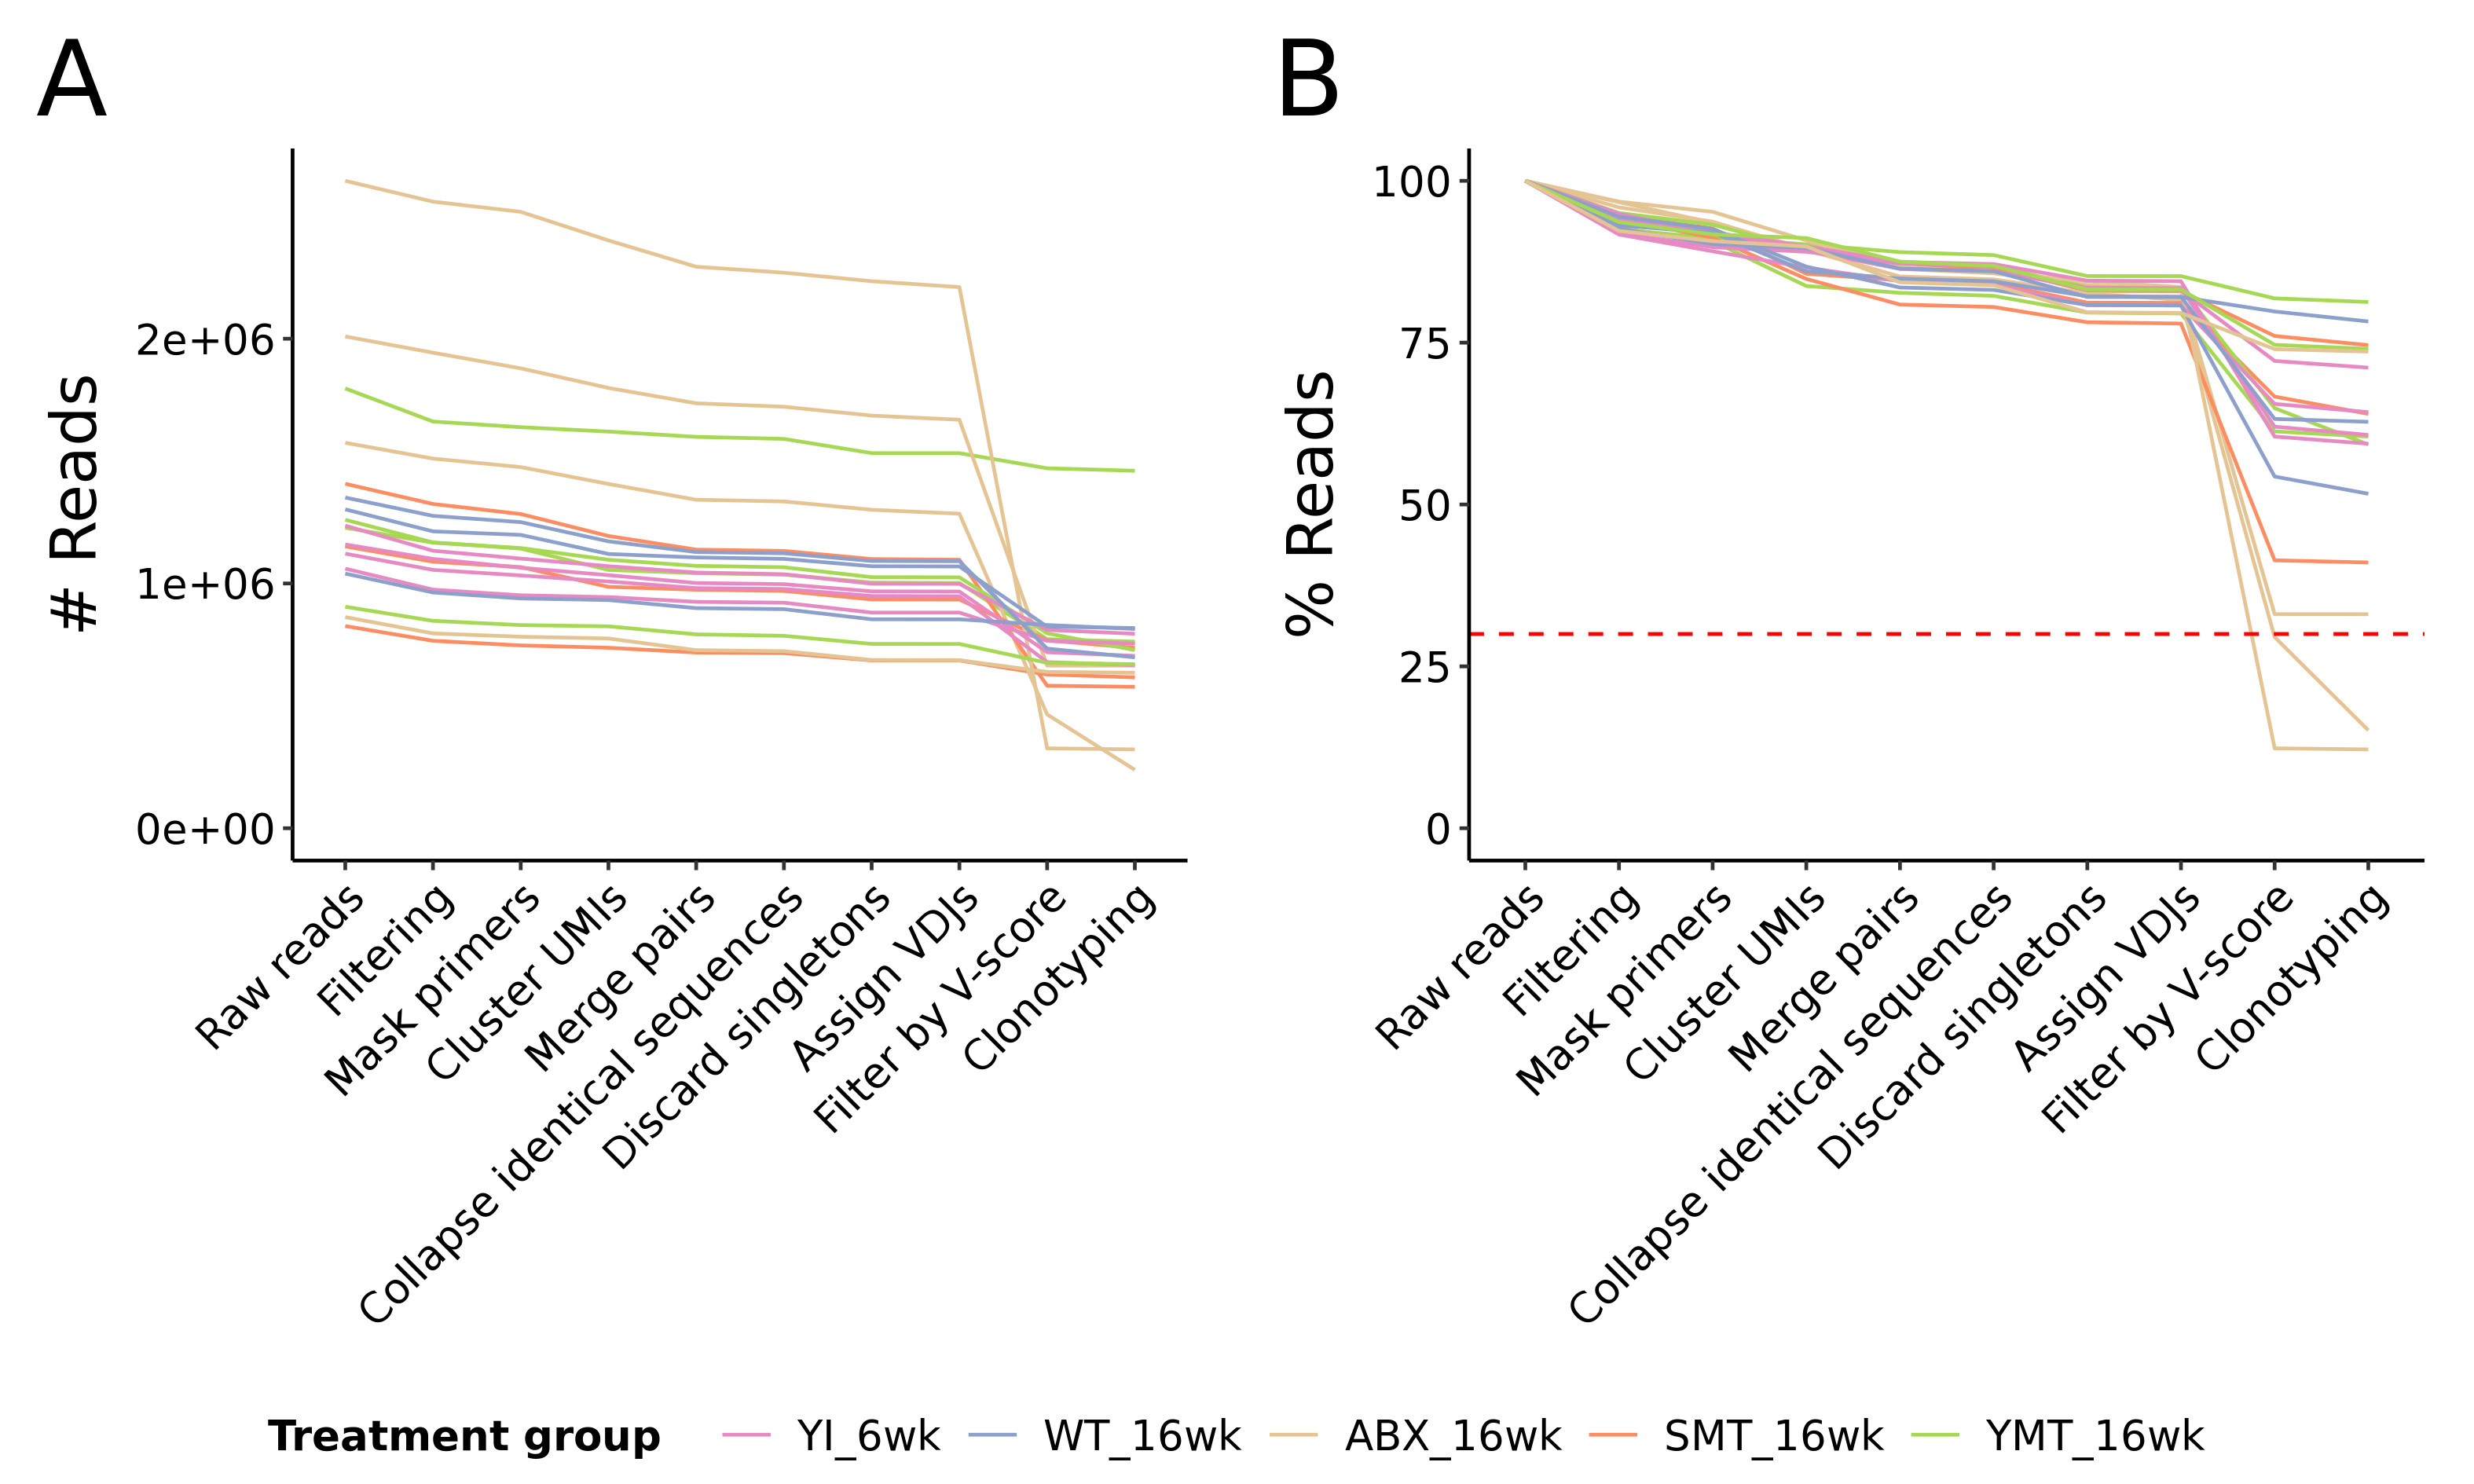
\includegraphics[width = 0.9\textwidth]{_Figures/png/gut-read-survival-all.png}
\begin{subfigure}{0em}
\phantomsubcaption{}
\label{fig:igseq-gut-read-survival-all-abs}
\end{subfigure}
\begin{subfigure}{0em}
\phantomsubcaption{}
\label{fig:igseq-gut-read-survival-all-rel}
\end{subfigure}
\caption{Absolute (A) and relative (B) read survival during pre-processing of the \igseq gut-microbiota-transfer dataset, up to and including clonotyping. The dotted red line in (B) indicates the 30\% read-survival cutoff, below which samples are discarded prior to downstream analysis.}
\label{fig:igseq-gut-read-survival-all}
\end{figure}

\begin{figure}
\centering
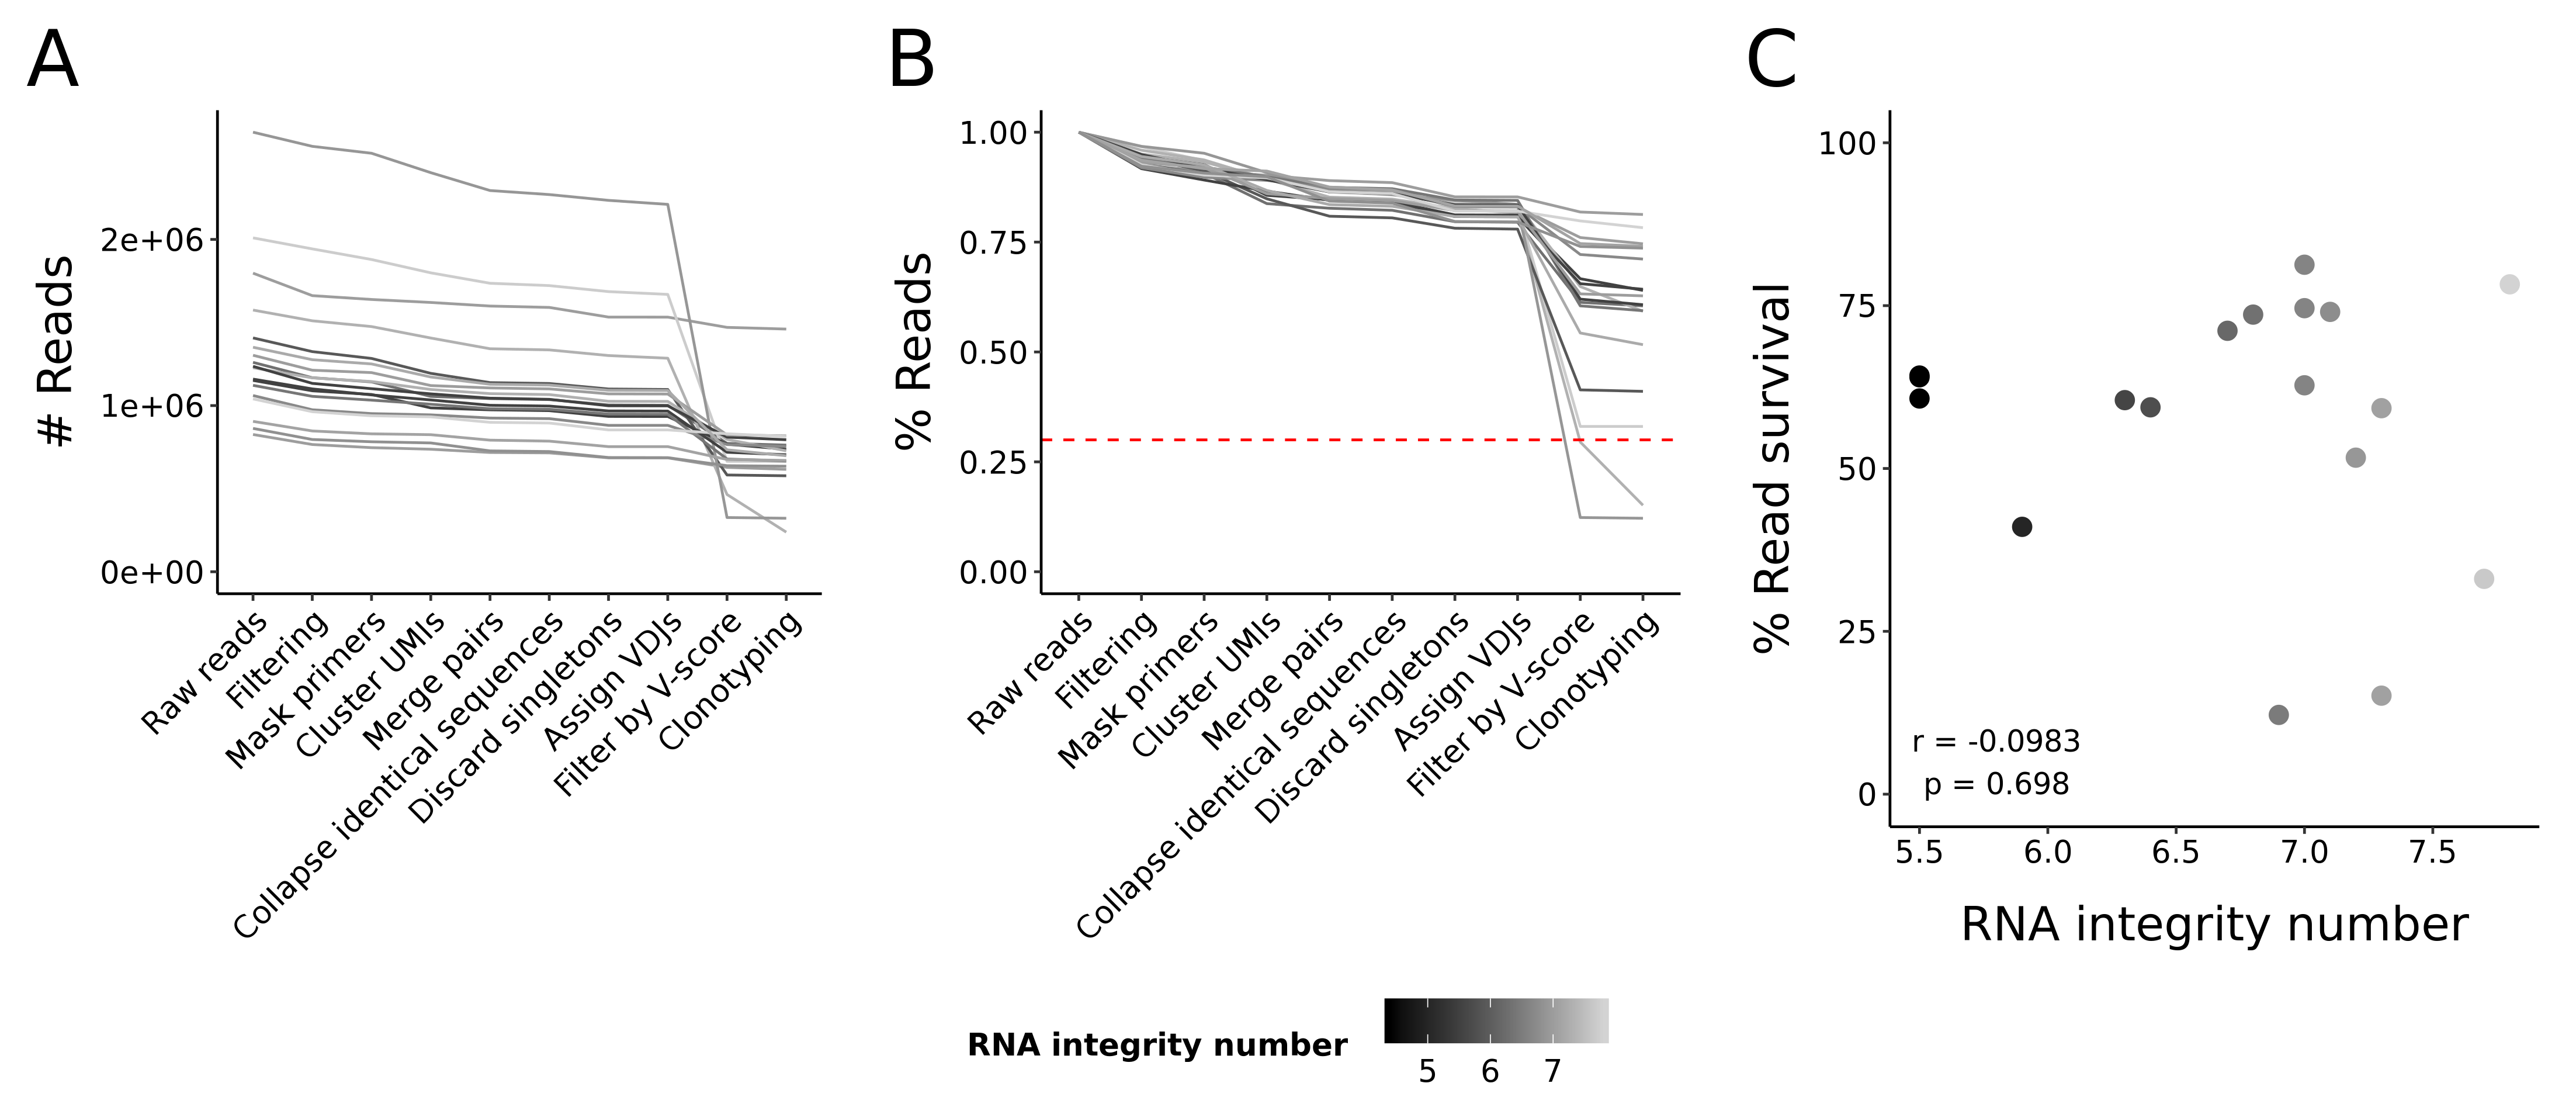
\includegraphics[width = \textwidth]{_Figures/png/gut-read-survival-all-rin.png}
\begin{subfigure}{0em}
\phantomsubcaption{}
\label{fig:igseq-gut-read-survival-all-rin-abs}
\end{subfigure}
\begin{subfigure}{0em}
\phantomsubcaption{}
\label{fig:igseq-gut-read-survival-all-rin-rel}
\end{subfigure}
\begin{subfigure}{0em}
\phantomsubcaption{}
\label{fig:igseq-gut-read-survival-all-rin-scatter}
\end{subfigure}
\caption[Relationship between RNA integrity and read survival in the gut \igseq dataset]{\textbf{Relationship between RNA integrity and read survival in the gut \igseq dataset:} (A-B) Absolute (A) and relative (B) read survival during pre-processing of the \igseq gut-microbiota-transfer dataset, up to and including clonotyping, coloured by the RNA integrity number of each input sample. The dotted red line in (B) indicates the 30\% read-survival cutoff, below which samples are discarded prior to downstream analysis. (C) Scatterplot of RNA integrity number \textit{versus} percentage read survival, up to and including clonotyping.}
\label{fig:igseq-gut-read-survival-all-rin}
\end{figure}


\begin{figure}
\centering
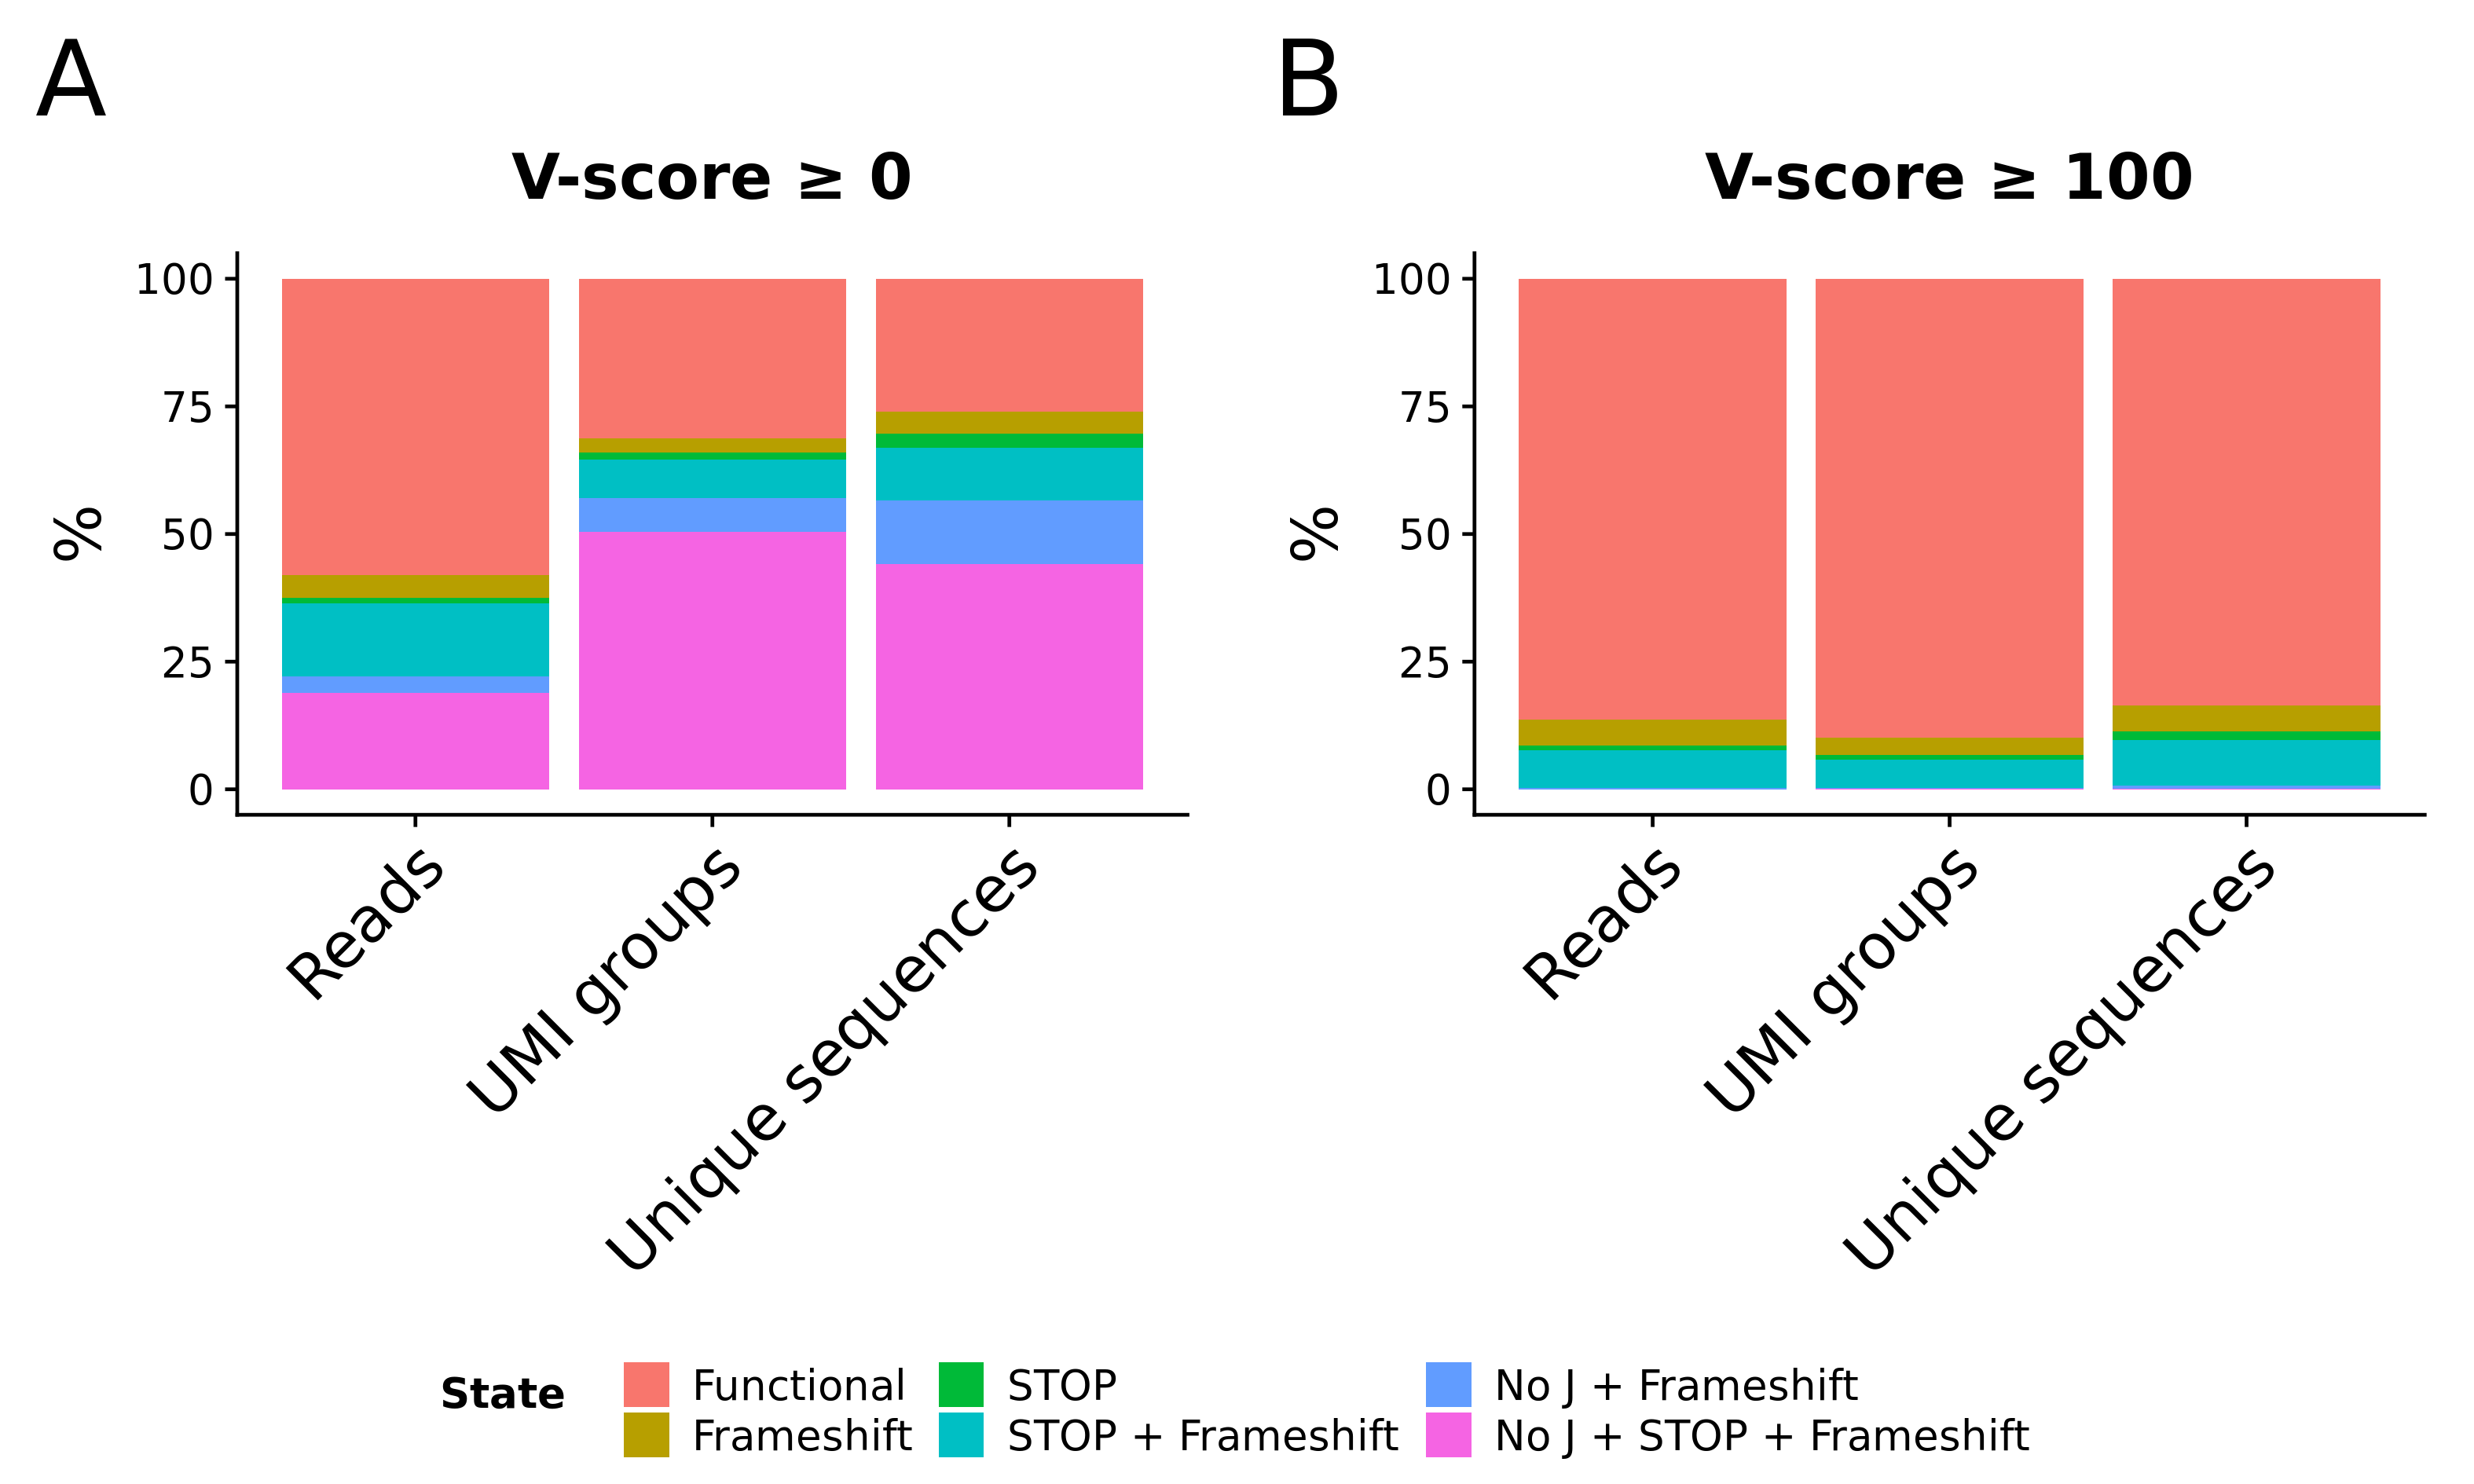
\includegraphics[width = 0.9\textwidth]{_Figures/png/gut-functional-prop}
\begin{subfigure}{0em}
\phantomsubcaption{}
\label{fig:igseq-gut-functional-prop-pre}
\end{subfigure}
\begin{subfigure}{0em}
\phantomsubcaption{}
\label{fig:igseq-gut-functional-prop-post}
\end{subfigure}
\caption{Proportion of input reads, UMI groups and unique sequences in the \igseq gut-microbiota-transfer dataset belonging to different (non)functional categories, before (A) and after (B) filtering on V-alignment score.}
\label{fig:igseq-gut-functional-prop}
\end{figure}

With two exceptions, the remaining samples from the gut microbiota transfer dataset exhibited a dramatically lower apparent clonal richness than either the pilot or ageing dataset, both in absolute terms (\Cref{fig:igseq-comparative-metrics-abs} -- with a median of \embed{_Figures/txt/igseq-gut-nclones-individual-med.txt} clones per individual compared to \embed{_Figures/txt/pilot-nclones-individual-med.txt} for the pilot dataset or \embed{_Figures/txt/ageing-nclones-individual-med.txt} for the ageing dataset) and relative to the number of UMI groups or unique sequences in each repertoire (\Cref{fig:igseq-comparative-metrics-rel}). This suggests, not entirely surprisingly, that killifish guts contain many fewer clones than whole-body killifish samples. However, the metrics presented in \Cref{fig:igseq-comparative-metrics} are strongly dependent on the size of each dataset: for example, even though the pilot dataset contains a subset of the individuals from the ageing dataset, their distributions in \Cref{fig:igseq-comparative-metrics} do not overlap.

In order to determine whether the apparent difference in clonal richness between the gut and other datasets is real, therefore, I performed rarefaction analysis, measuring the number of clones in repeated downsamplings of UMI groups from each dataset, along with the P20. % TODO: Already explained P20 above?
The results for the rarefied clonal counts (\Cref{fig:igseq-rarefied-clone-counts}) confirm the results from \Cref{fig:igseq-comparative-metrics-abs}: at any given downsampling size, the great majority of repertoires from the gut dataset contain far fewer clones than the repertoires in the pilot or ageing datasets. Concordantly, the gut repertoires also show a much greater degree of dominance by the largest clones in each repertoire, with over 85\% of gut samples exhibiting greater asymptotic P20 than over 90\% of ageing or pilot individuals and over 65\% exhibiting higher asymptotic P20 than any sample in the other experiments. In both cases (clonal counts and P20), a small minority of individuals deviate strongly from the general trend, exhibiting clonal counts and P20 values more consistent with those seen in the pilot and ageing experiments; however, only one individual (1412, from the 6-week-old untreated group) is an outlier in both clonal count and P20 value.

\begin{figure}
\centering
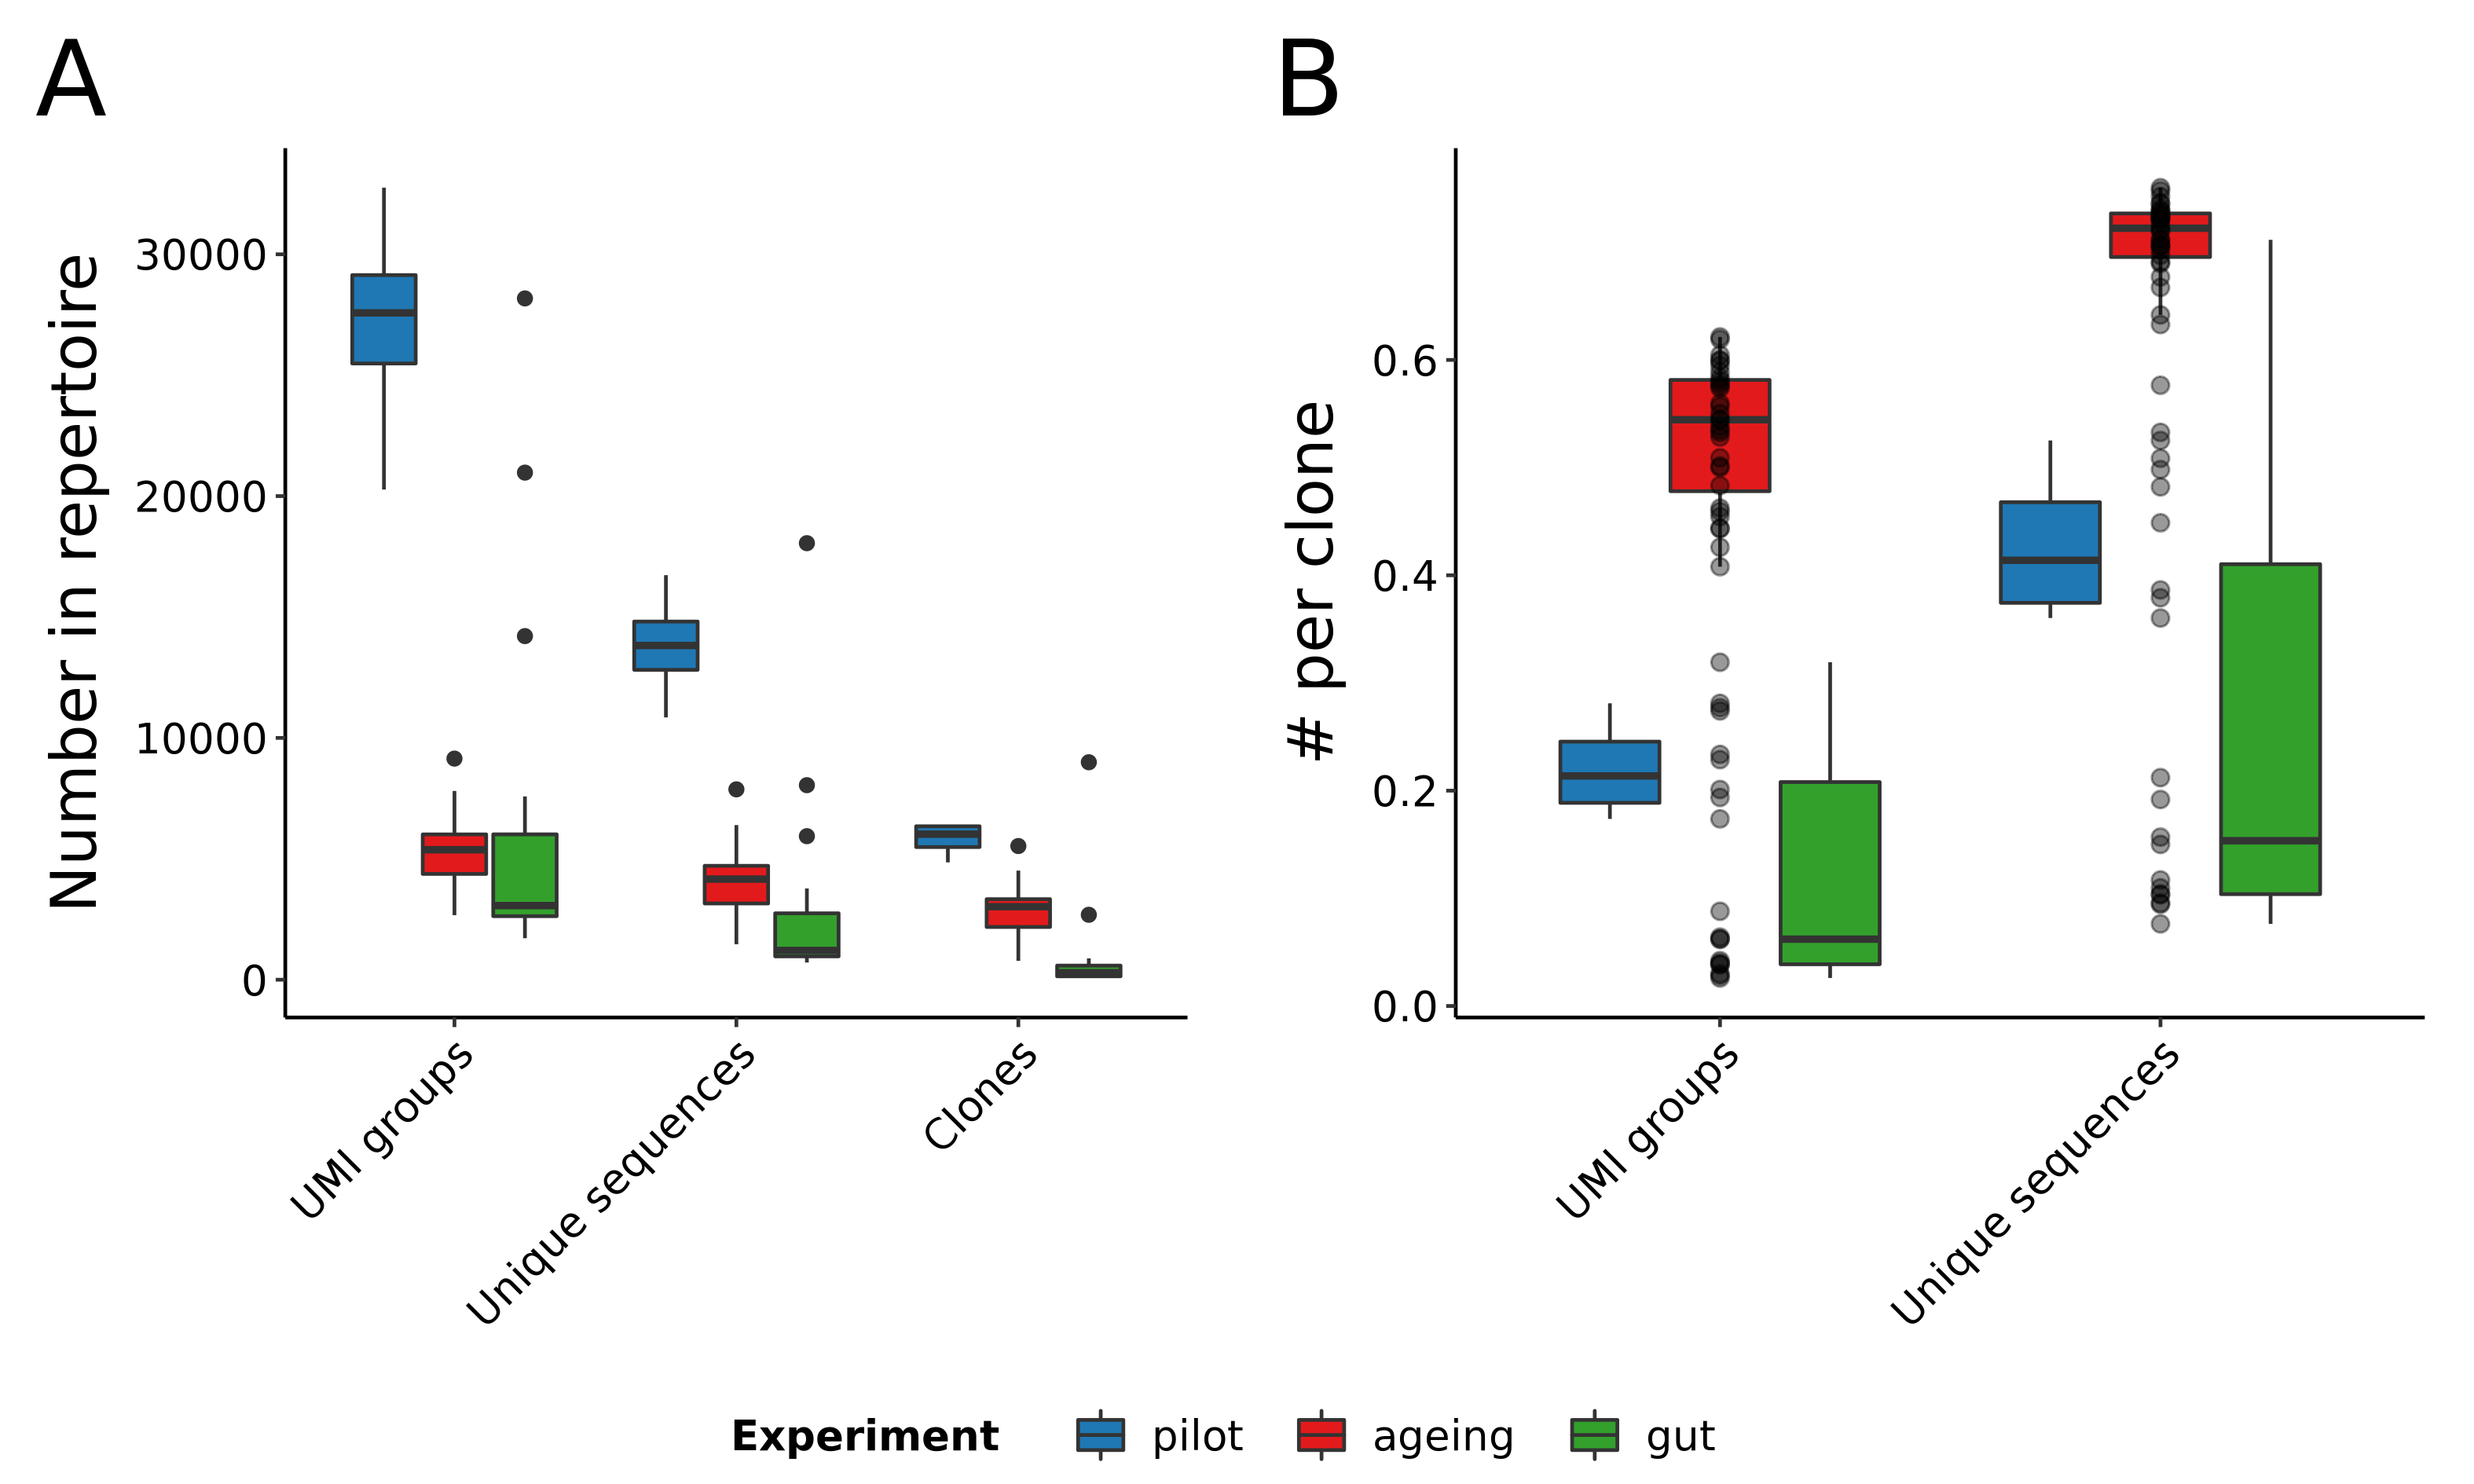
\includegraphics[width = 0.9\textwidth]{_Figures/png/igseq-comparative-metrics}
\begin{subfigure}{0em}
\phantomsubcaption{}
\label{fig:igseq-comparative-metrics-abs}
\end{subfigure}
\begin{subfigure}{0em}
\phantomsubcaption{}
\label{fig:igseq-comparative-metrics-rel}
\end{subfigure}
\caption{Absolute (A) and relative (B) read survival during pre-processing of the \igseq gut-microbiota-transfer dataset, up to and including clonotyping. The dotted red line in (B) indicates the 30\% read-survival cutoff, below which samples are discarded prior to downstream analysis.}
\label{fig:igseq-comparative-metrics}
\end{figure}

\begin{figure}
\centering
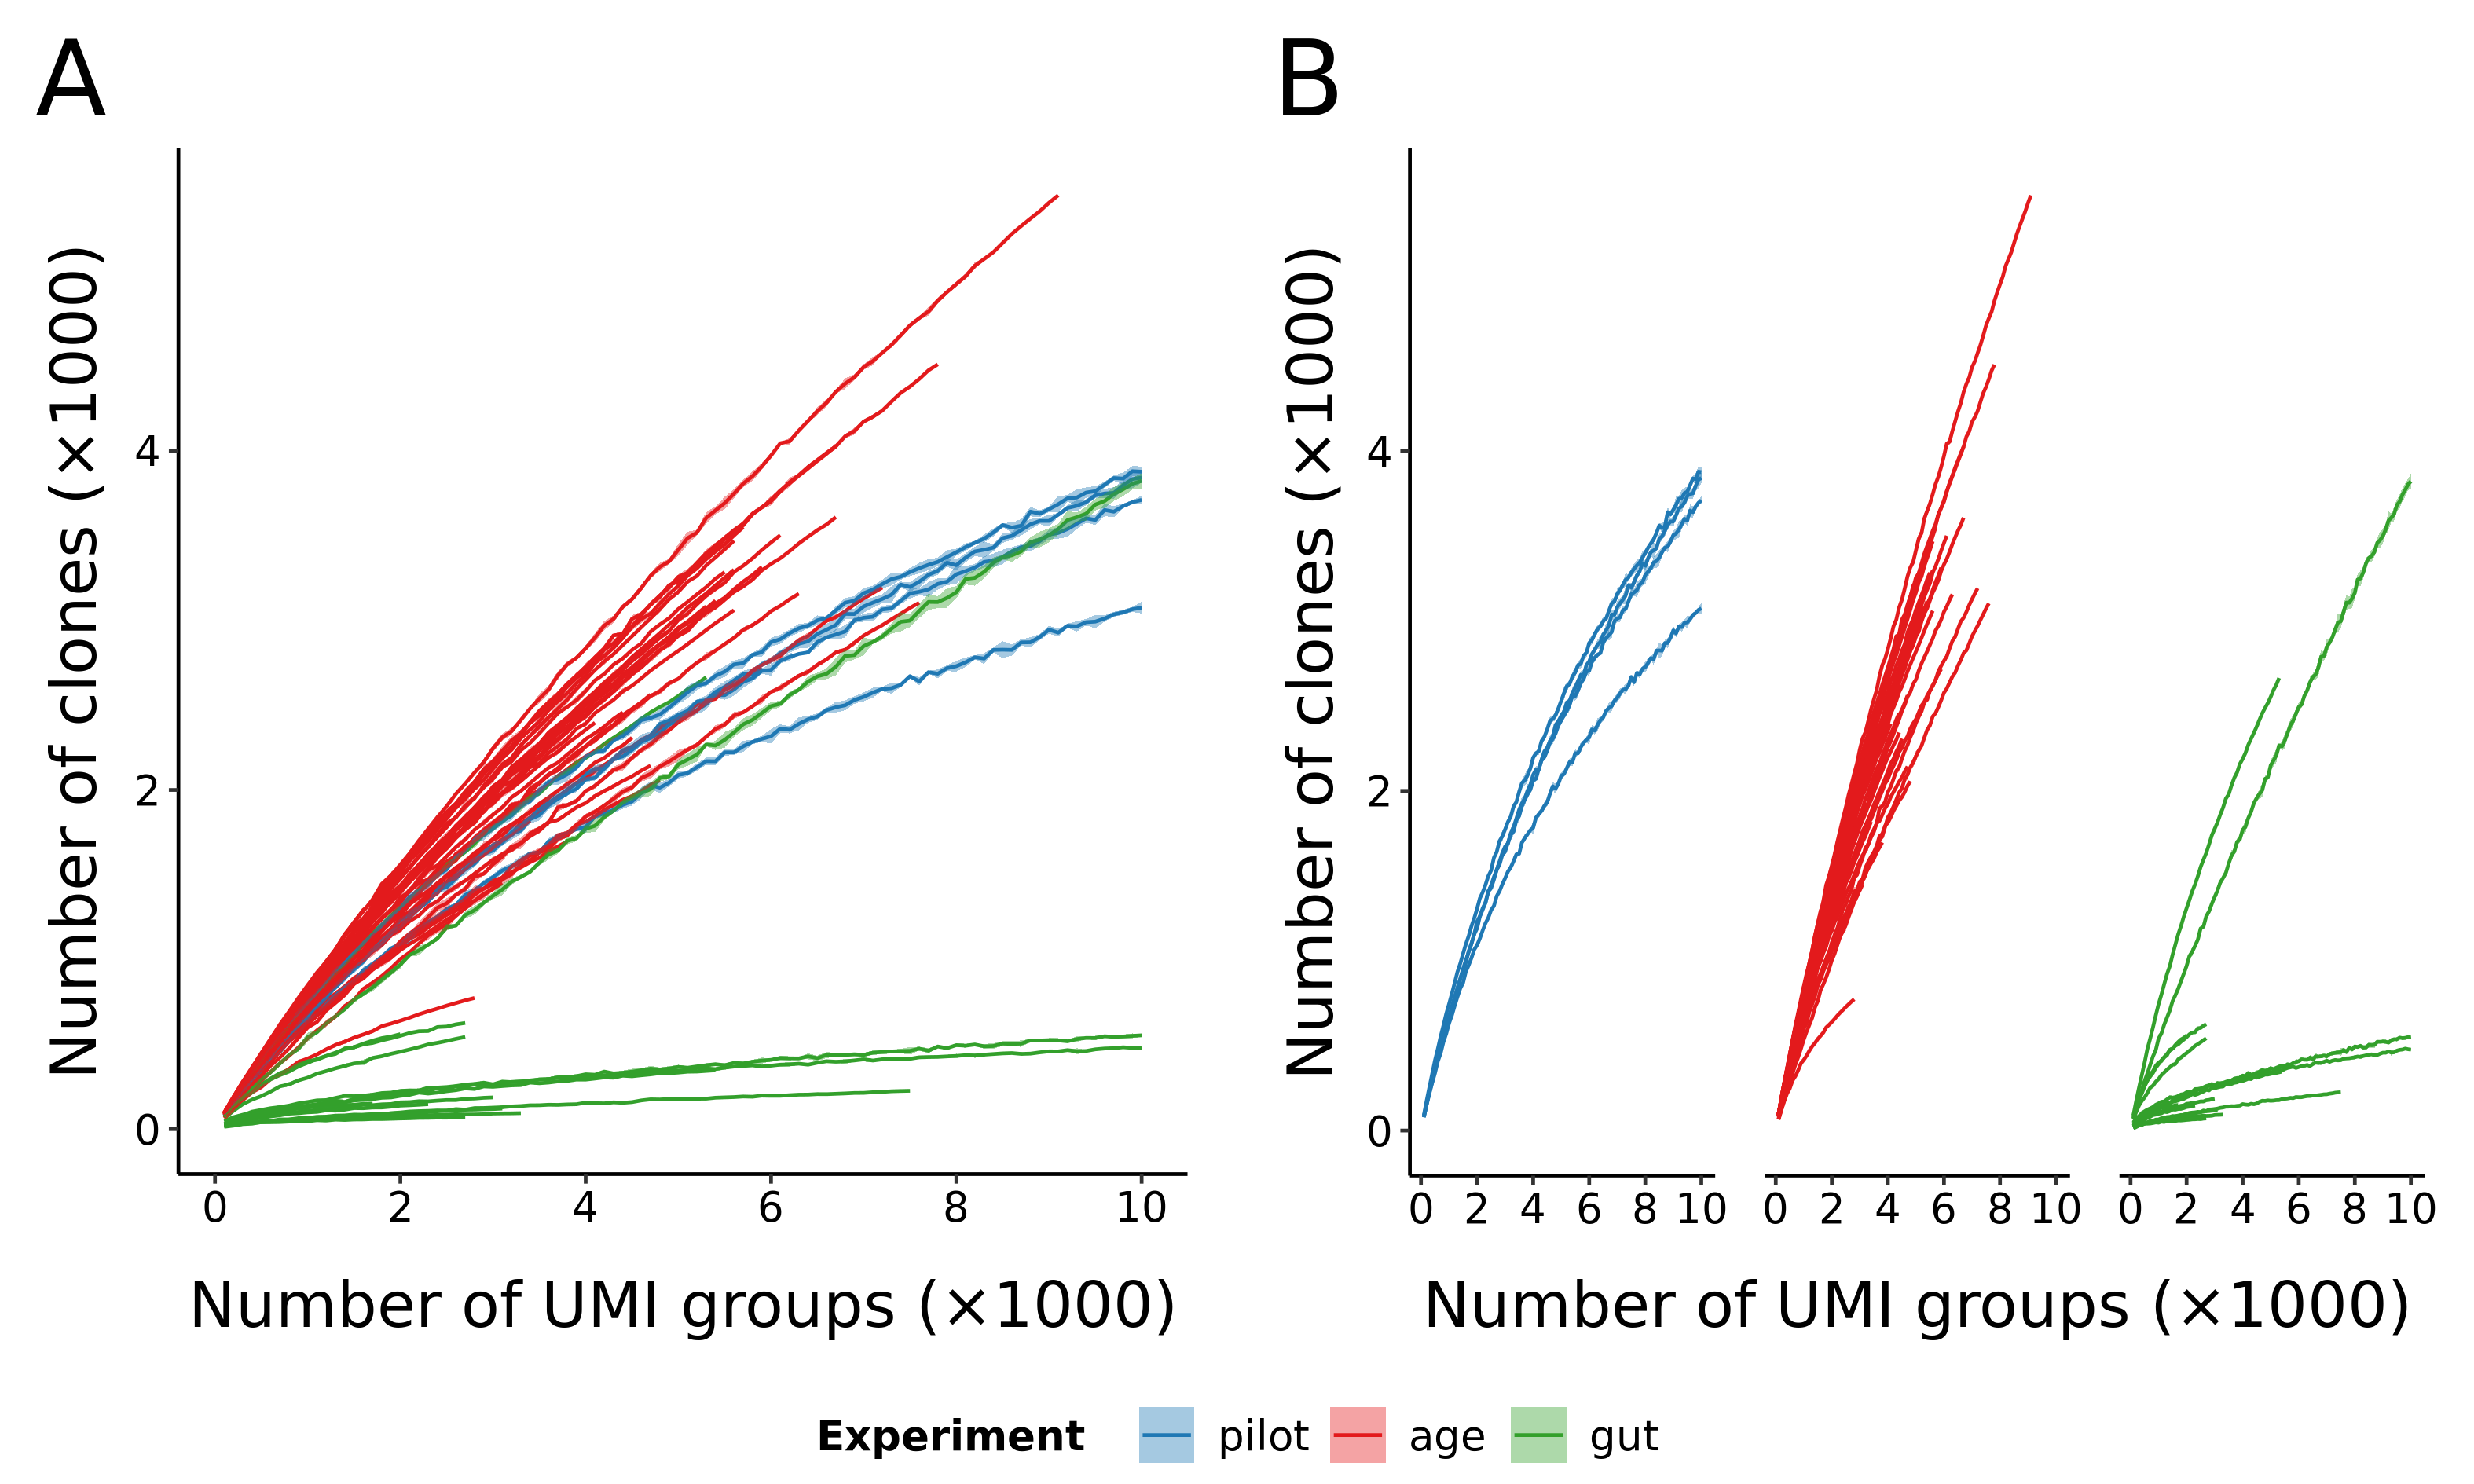
\includegraphics[width = 0.9\textwidth]{_Figures/png/igseq-rarefied-clone-counts}
\begin{subfigure}{0em}
\phantomsubcaption{}
\label{fig:igseq-rarefied-clone-counts-all}
\end{subfigure}
\begin{subfigure}{0em}
\phantomsubcaption{}
\label{fig:igseq-rarefied-clone-counts-facets}
\end{subfigure}
\caption{Rarefaction analysis of clonal counts in turquoise killifish repertoires from the \igseq pilot, ageing and gut-microbiota-transfer experiments, displayed together (B) and separately by experiment (B). Lines and shaded regions indicate the mean and standard deviation, respectively, over five replicates per sample size.}
\label{fig:igseq-rarefied-clone-counts}
\end{figure}
% TODO: Increase number of iterations (20?)

\begin{figure}
\centering
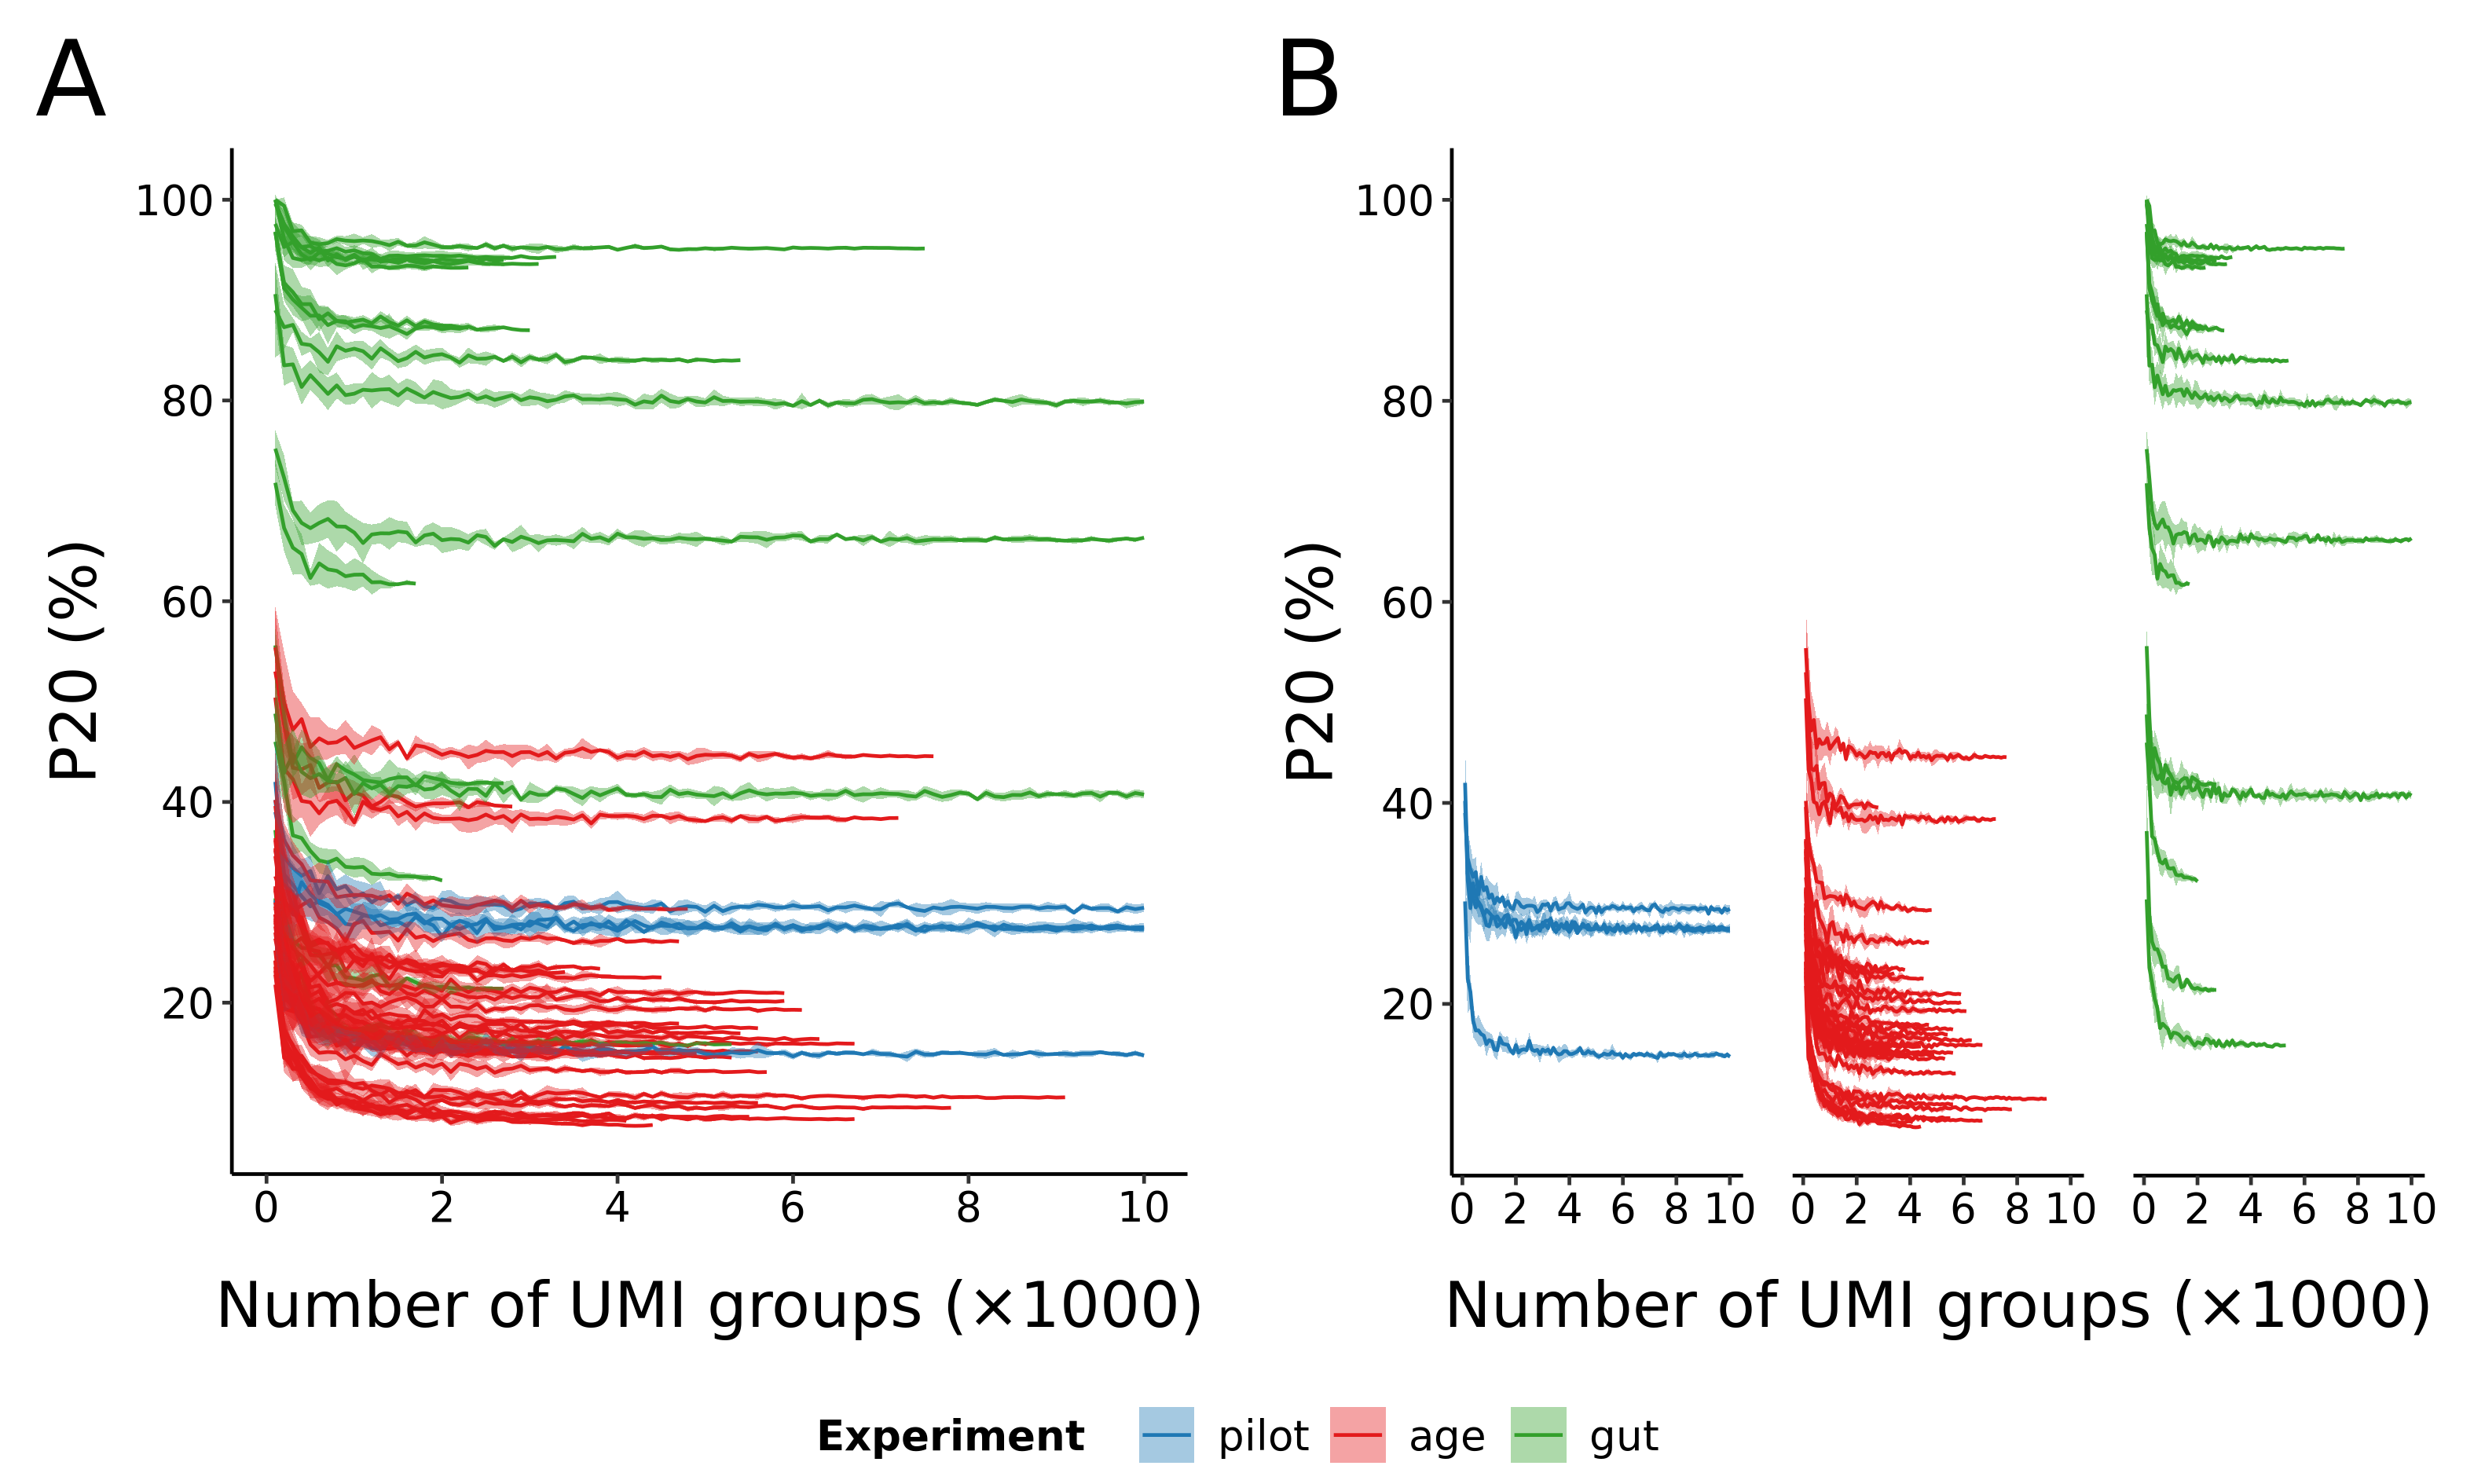
\includegraphics[width = 0.9\textwidth]{_Figures/png/igseq-rarefied-clone-p20}
\begin{subfigure}{0em}
\phantomsubcaption{}
\label{fig:igseq-rarefied-clone-p20-all}
\end{subfigure}
\begin{subfigure}{0em}
\phantomsubcaption{}
\label{fig:igseq-rarefied-clone-p20-facets}
\end{subfigure}
\caption{Rarefaction analysis of the proportion of each turquoise killifish repertoire occupied by the twenty largest clones (P20) in the \igseq pilot, ageing and gut-microbiota-transfer experiments, displayed together (A) and separately by experiment (B). Lines and shaded regions indicate the mean and standard deviation, respectively, over five replicates per sample size.}
\label{fig:igseq-rarefied-clone-p20}
\end{figure}
% TODO: Increase number of iterations (20?)

The killifish gut repertoire therefore exhibits not only a much lower clonal richness than the whole-body repertoire, but also in most cases a much greater degree of domination by the largest few clones. As briefly observed above, this is not altogether surprising: the whole-body repertoire includes clones from primary haematopoietic organs like the head kidney, which would be expected to contain many more small, \naive clones than a secondary lymphoid organ like the gut. In addition, as the B-cells in the gut are in close proximity and interaction with the gut microbiota, it is not surprising that they should show a much greater degree of clonal expansion and hence a larger average P20. Nevertheless, it is useful to confirm these phenomena, both as a sanity check about the quality of these datasets and because it may have important implications for the results of downstream analyses of the gut dataset.

% TODO: Zipf parameters? Other clonal measures?

The clonal alpha-diversity spectra for the gut dataset are shown in \Cref{fig:igseq-gut-clone-diversity-alpha}. At all diversity orders, there is a clear and drastic difference between the young (6-week-old) and old (16-week-old) groups, while the different 16-week-old treatment groups do not appear to show a strong difference in diversity. These observations are confirmed by statistical comparison of the distributions of individual diversity measurements at different diversity orders, which indicate highly significant differences in clonal repertoire diversity between young and old guts across the diversity spectrum (\Cref{fig:igseq-gut-clone-diversity-solo-age}), but no difference between treatment groups (\Cref{fig:igseq-gut-clone-diversity-solo-groups}). A similar pattern is observed for V/J-usage diversity (\Cref{fig:igseq-gut-VJ-diversity-alpha}), with a large and significant difference between young and old cohorts at many different diversity orders (\Cref{fig:igseq-gut-VJ-diversity-solo-age}) but no significant differences between 16-week-old treatment groups (\Cref{fig:igseq-gut-VJ-diversity-solo-groups}).

In terms of beta-diversity, the Hill-spectrum results (\Cref{fig:igseq-gut-VJ-diversity-beta}) are equivocal, with large differences in diversity between age groups observed at intermediate diversity orders (c. 1 to 2.5) but not at very low or very high orders (\Cref{fig:igseq-gut-VJ-diversity-beta-age}). Different treatment groups, meanwhile, exhibit very different patterns of beta diversity at higher orders (\Cref{fig:igseq-gut-VJ-diversity-beta-groups}), but not in any clear pattern: the antibiotic-treated and same-age-transfer groups show very high high-order beta diversity, indicating nearly maximal difference between individuals in their VJ-usage profiles, while the untreated and same-age-transfer groups show much lower between-individual variablity. To more closely investigate differences in inter-individual variability between sample groups, I again computed repertoire dissimilarity index (RDI) distances between each pair of individual repertoires in the dataset, and visualised the results by age cohort (\Cref{fig:igseq-gut-rdi-VJ-individual-age}) and treatment group (\Cref{fig:igseq-gut-rdi-VJ-individual-group}). The results again indicate large differences in VJ-usage variability between young and old gut repertoires in the turquoise killifish, with young samples clustering much more closely together (\Cref{fig:igseq-gut-rdi-VJ-individual-age-pcoa-facet}) and exhibiting consequently much lower pairwise RDI distances (\Cref{fig:igseq-gut-rdi-VJ-individual-age-groupdist-all,fig:igseq-gut-rdi-VJ-individual-age-groupdist-nn}); conversely, there is no significant difference in RDI distribution between the different 16-week-old treatment groups, indicating that the different groups are similar in their inter-individual variability. These RDI results contrast markedly with the differences in beta-spectra observed in \Cref{fig:igseq-gut-VJ-diversity-beta-groups}, suggesting that the latter may not be reliable measures of significant differences in intra-group variablity when sample sizes are small.

\begin{figure}
\centering
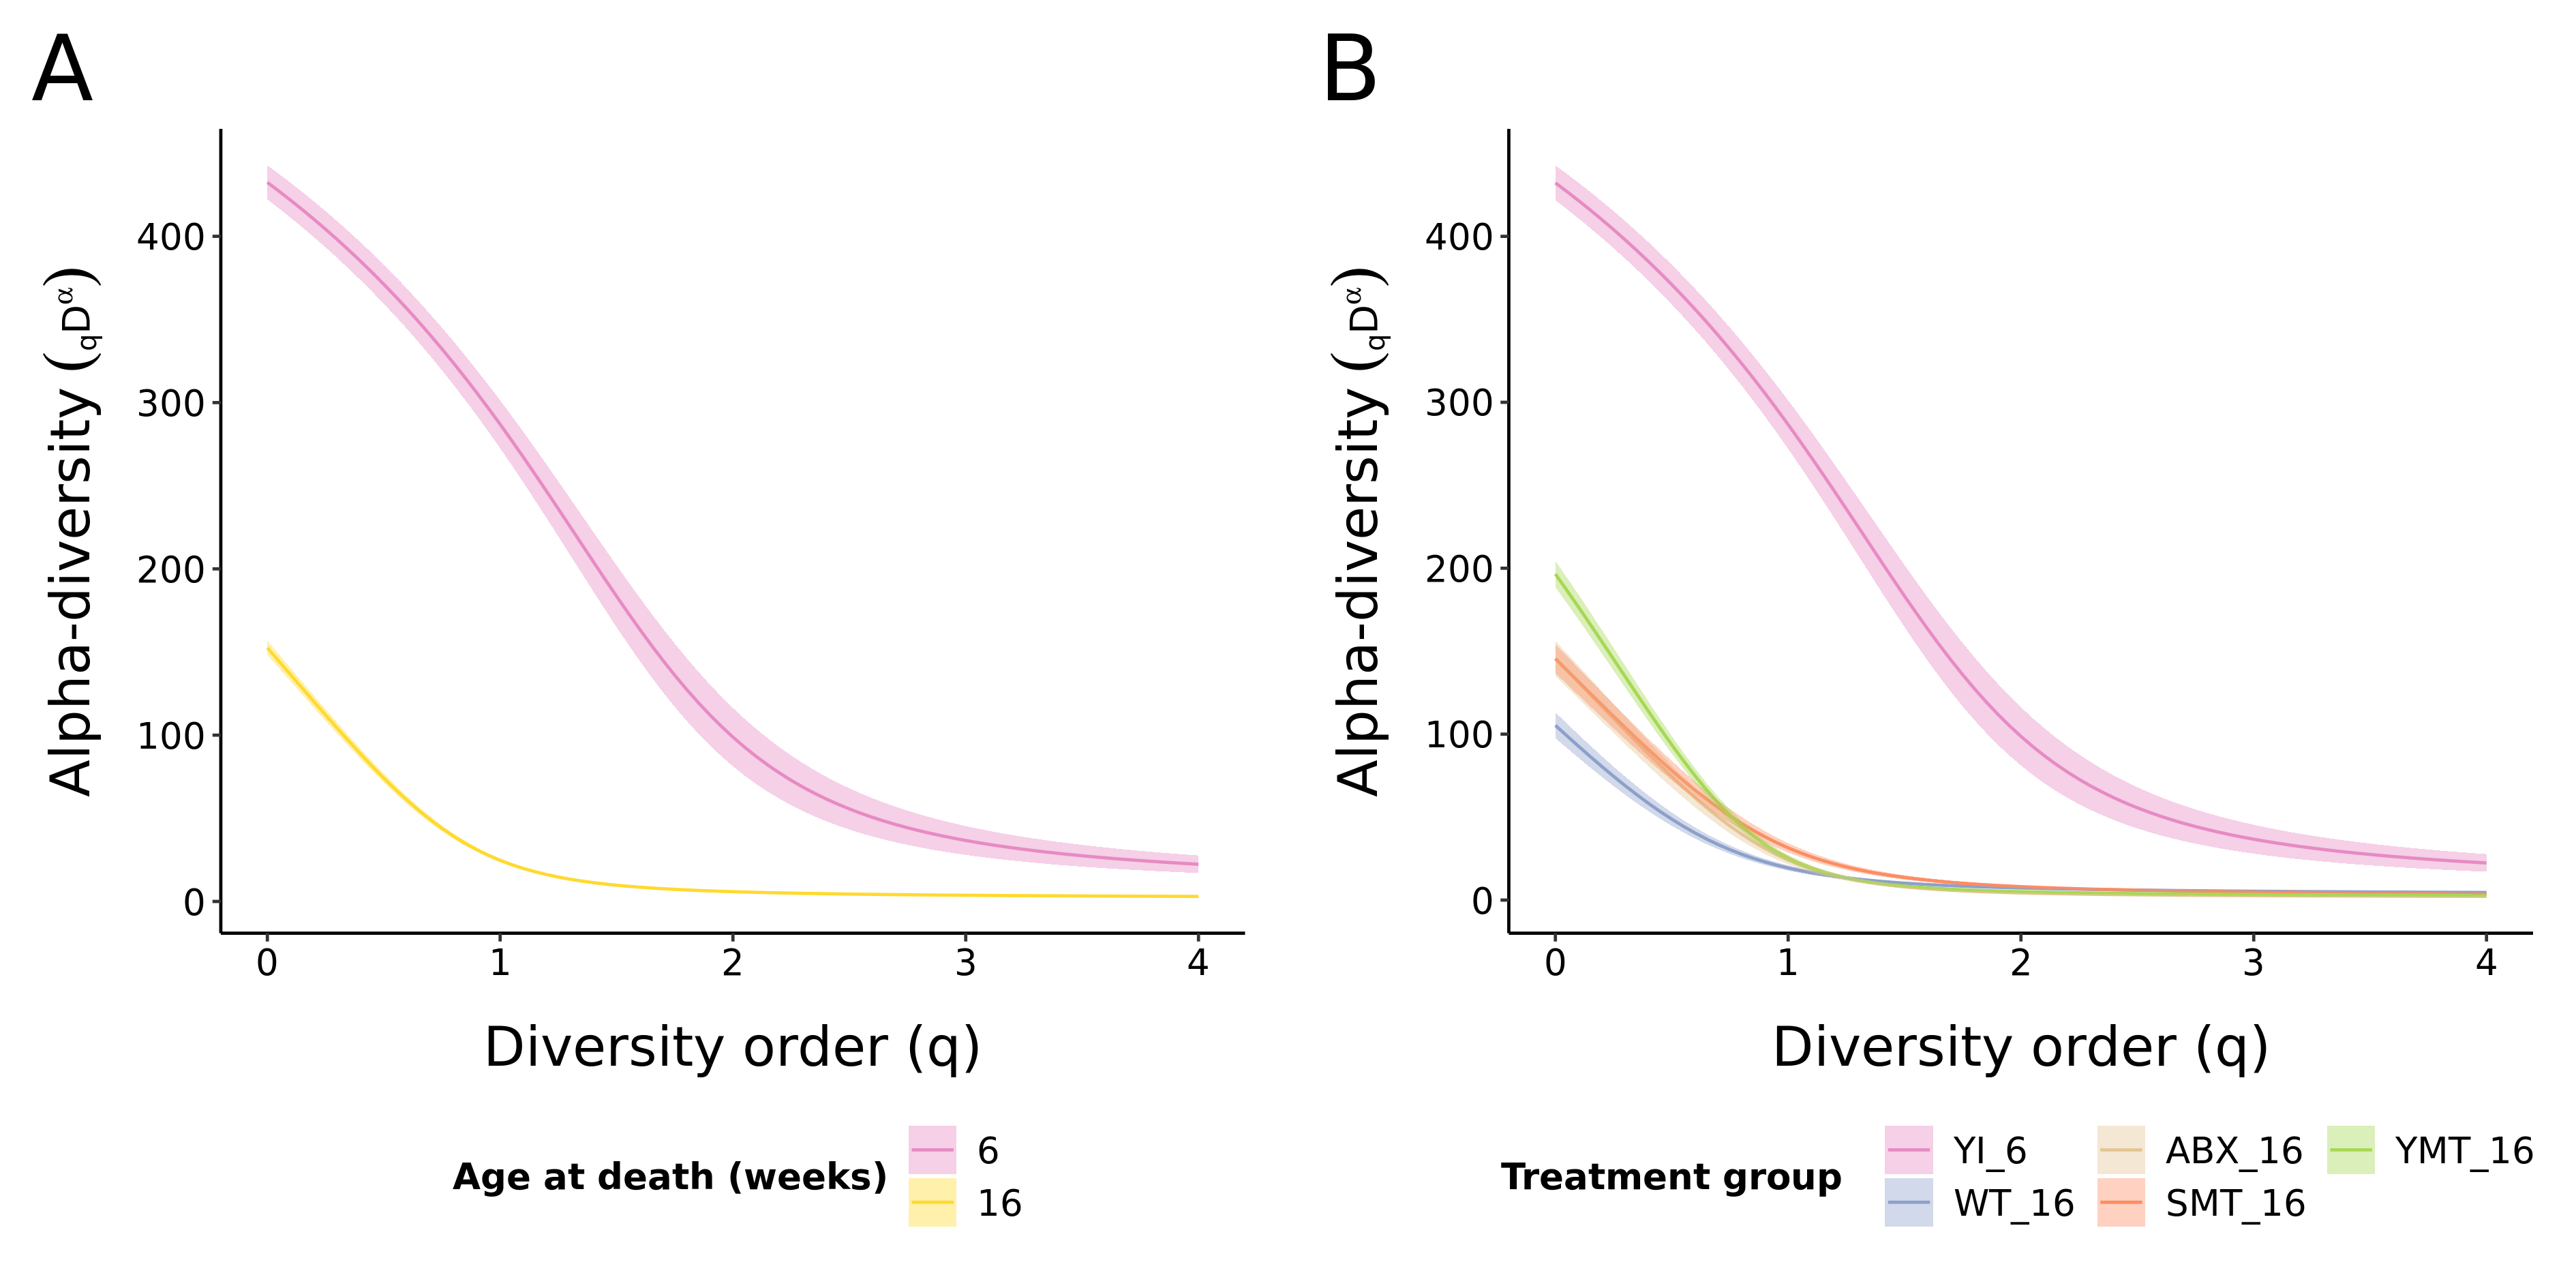
\includegraphics[width = 0.9\textwidth]{_Figures/png/igseq-gut-clone-diversity-alpha}
\begin{subfigure}{0em}
\phantomsubcaption{}
\label{fig:igseq-gut-clone-diversity-alpha-age}
\end{subfigure}
\begin{subfigure}{0em}
\phantomsubcaption{}
\label{fig:igseq-gut-clone-diversity-alpha-groups}
\end{subfigure}
\caption{Bootstrapped alpha-diversity spectra of clone sizes for each age (A) age group and (B) treatment group in the \igseq gut dataset, as measured by number of unique sequences per clone.}
\label{fig:igseq-gut-clone-diversity-alpha}
\end{figure}

\begin{figure}
\centering
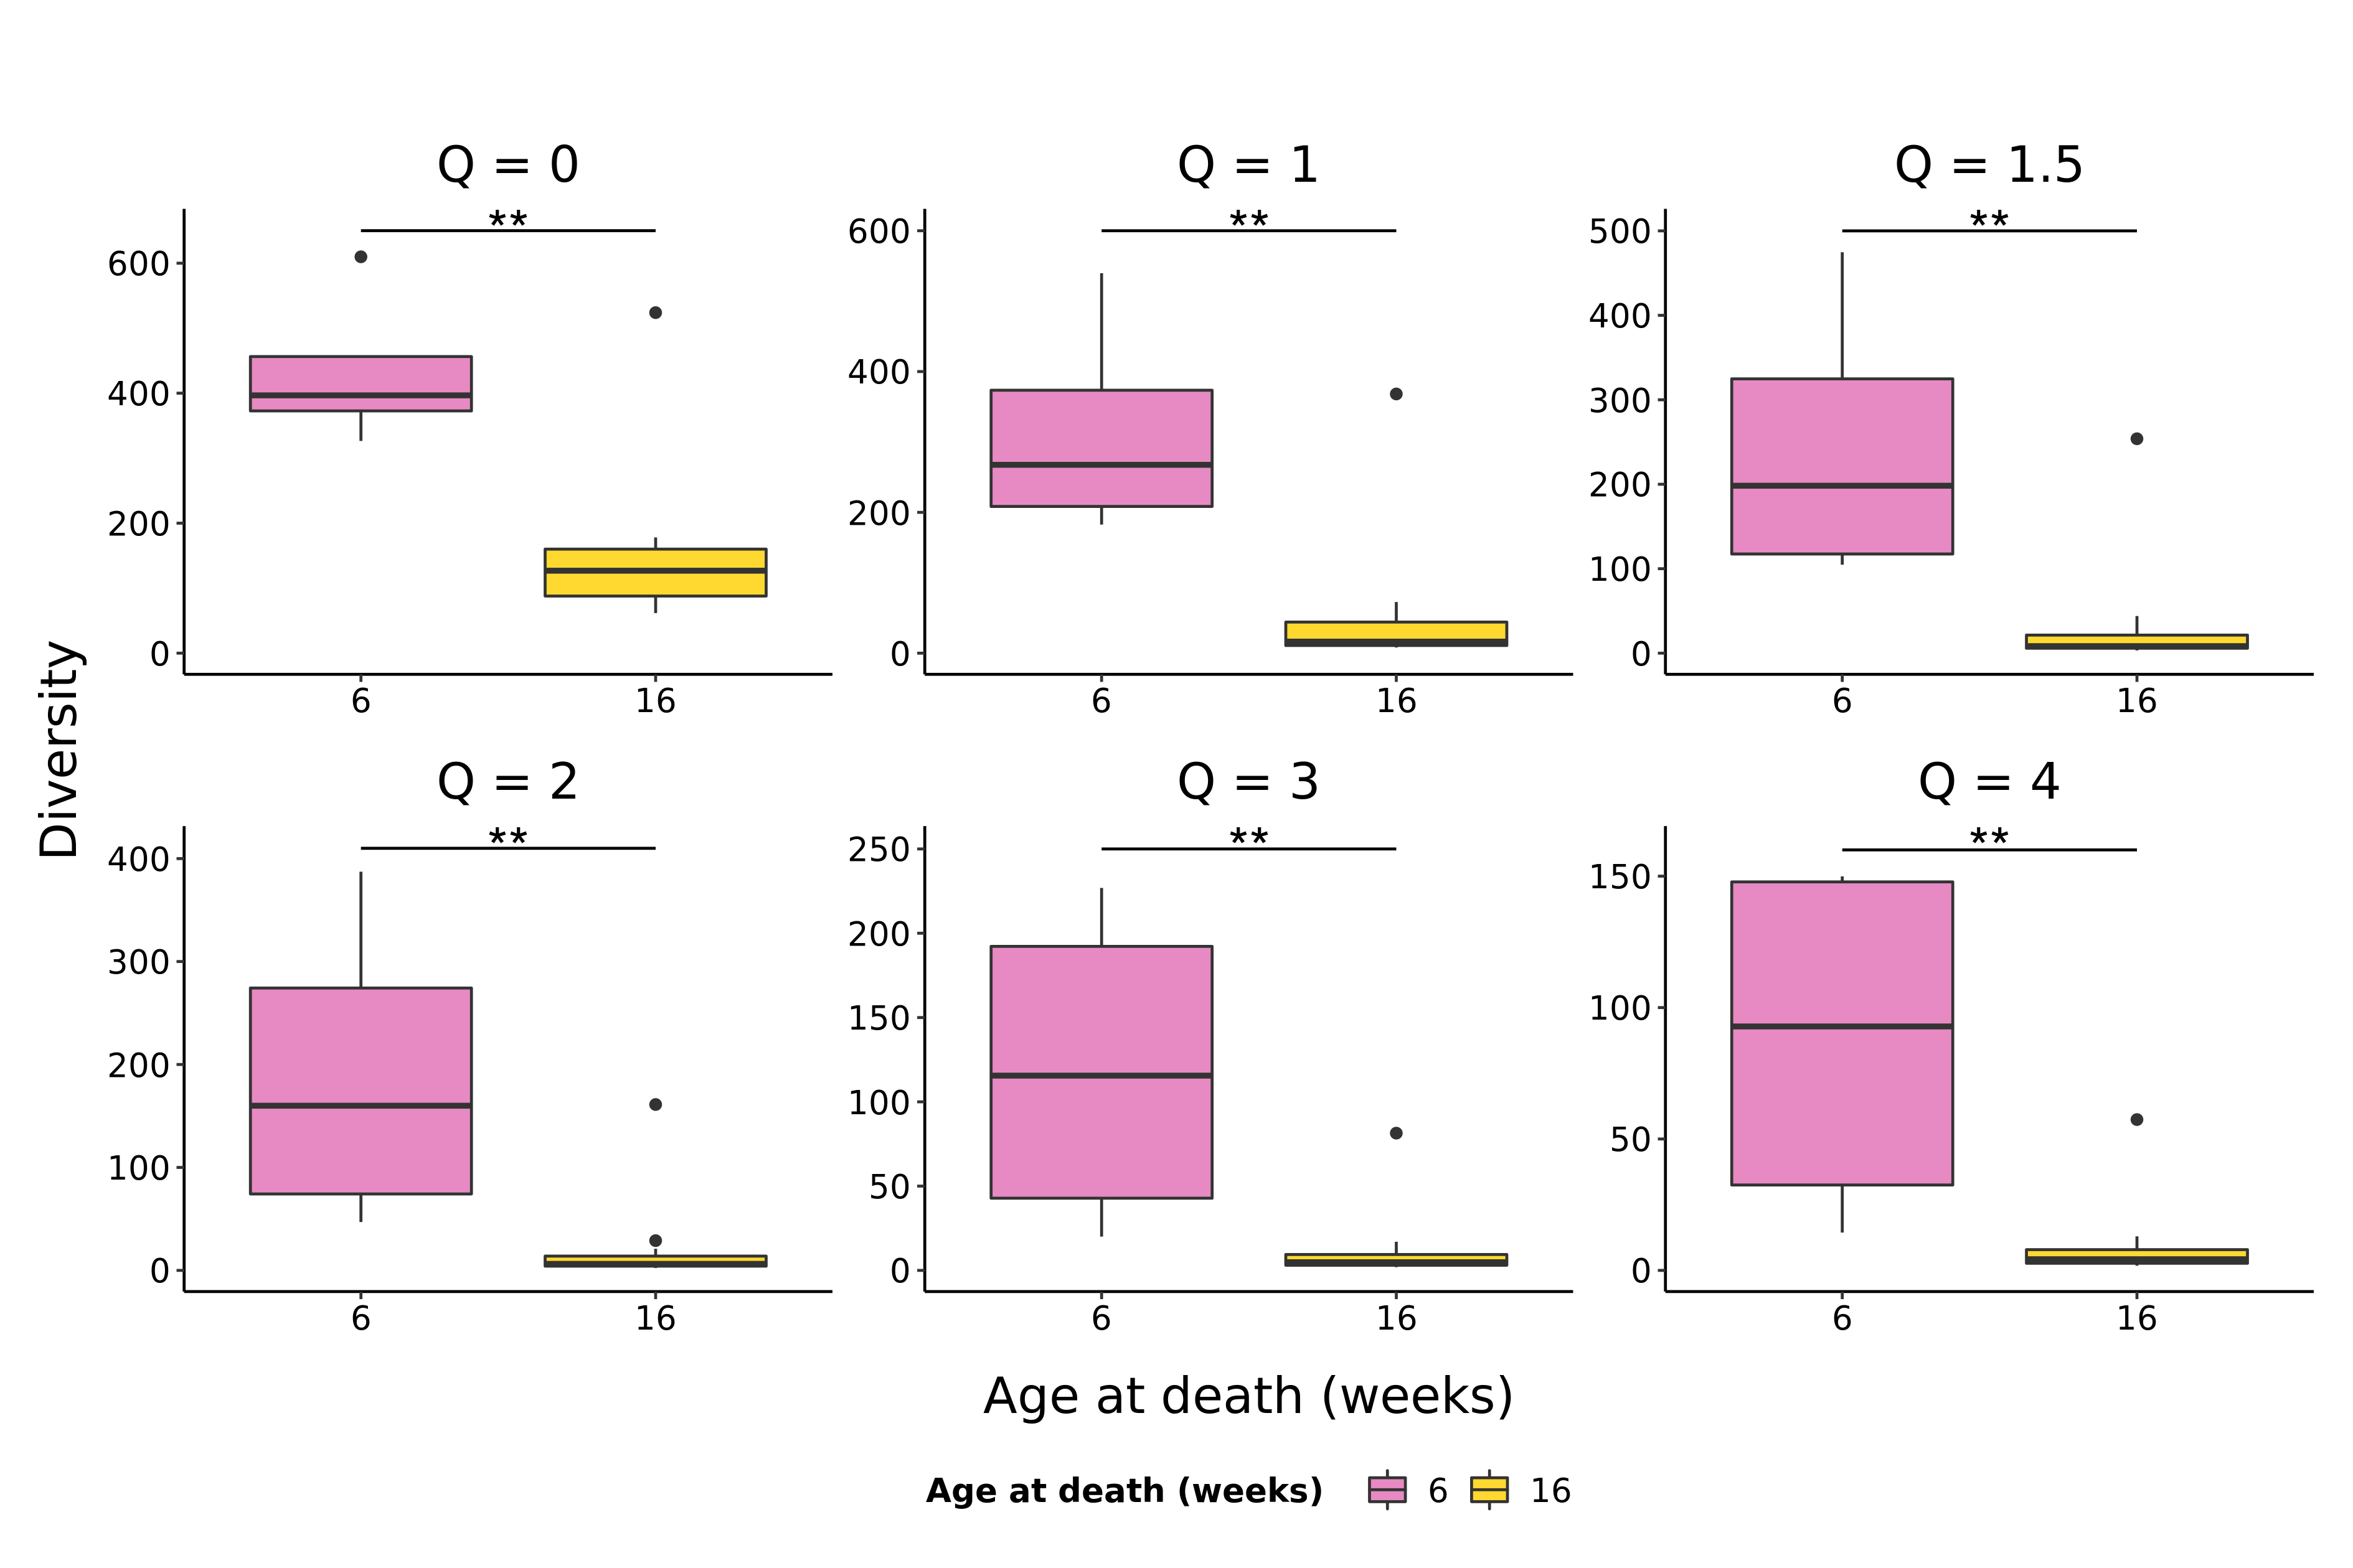
\includegraphics[width = 0.9\textwidth]{_Figures/png/igseq-gut-clone-diversity-solo-age}
\caption{Boxplots of \textit{clonal} Hill diversity values for the antibody repertoires of individuals of each age group in the \igseq gut dataset at a sample of diversity orders. Pairwise $p$-values are computed using nonparametric Mann–Whitney U tests ($*: 0.01 < p \leq 0.05;~**: 0.001 < p \leq 0.01;~***: p \leq 0.001$).}
\label{fig:igseq-gut-clone-diversity-solo-age}
\end{figure}

\begin{figure}
\centering
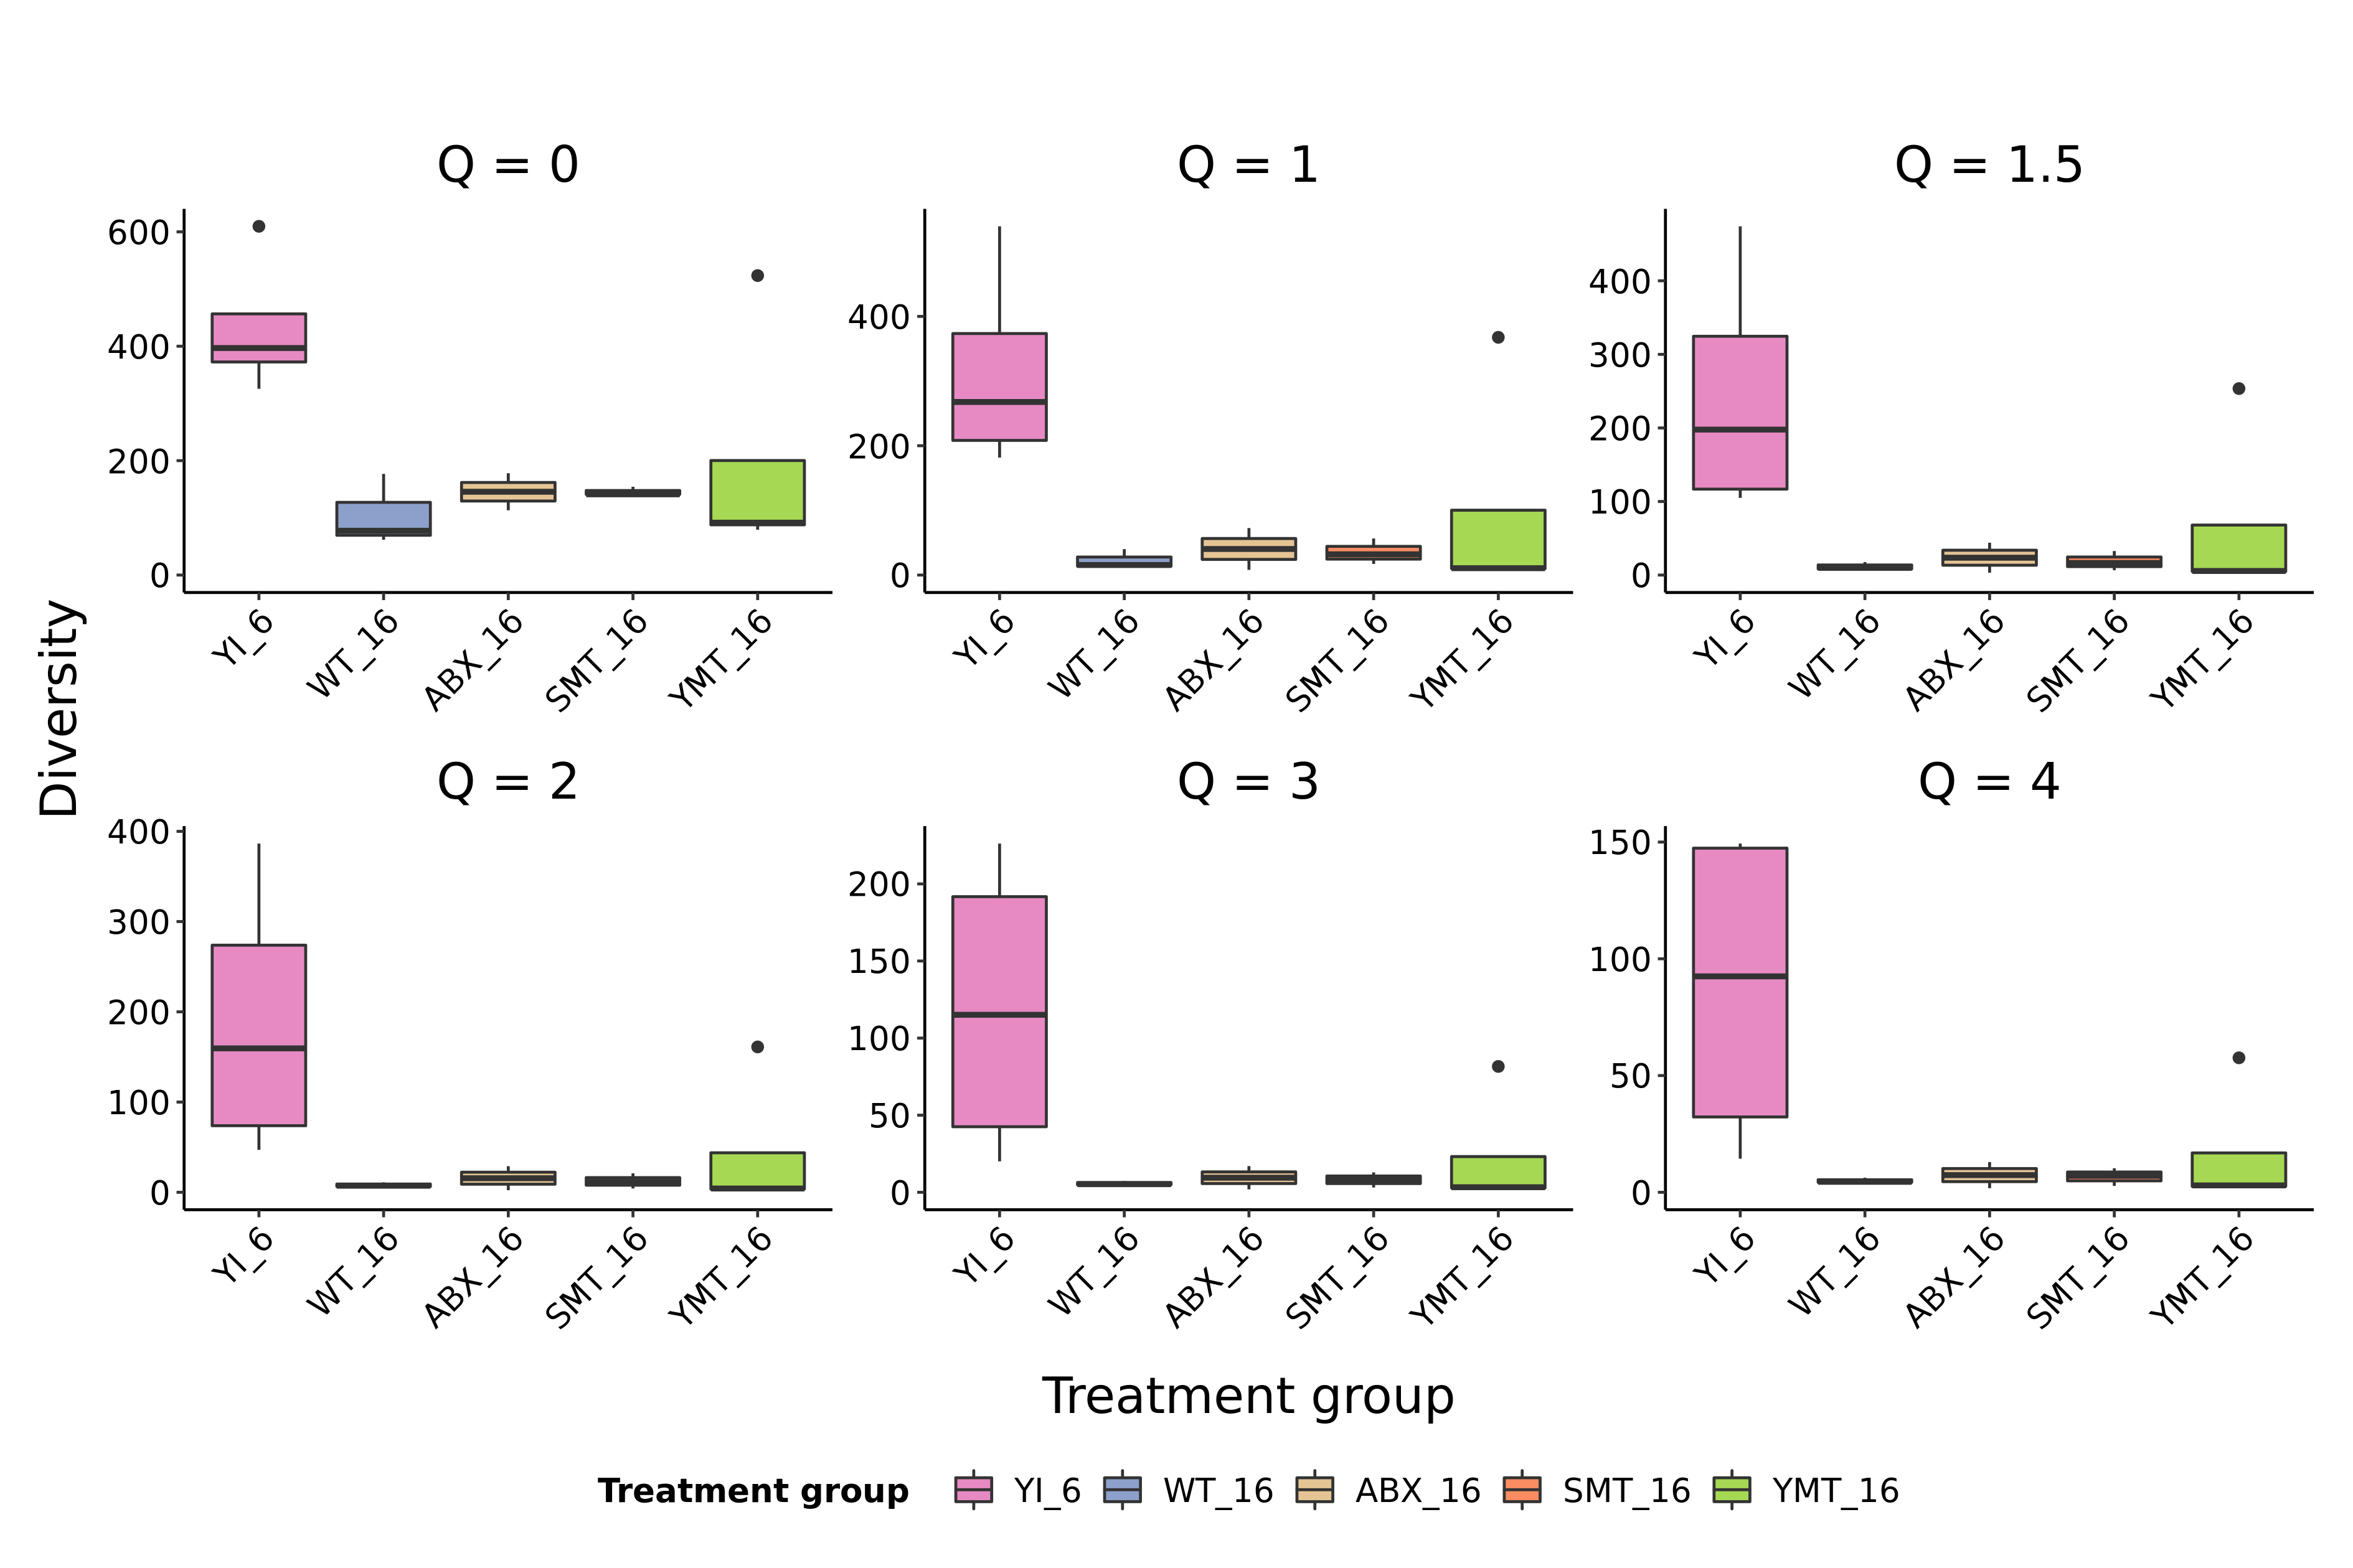
\includegraphics[width = 0.9\textwidth]{_Figures/png/igseq-gut-clone-diversity-solo-groups}
\caption{Boxplots of \textit{clonal} Hill diversity values for the antibody repertoires of individuals of each treatment group in the \igseq gut dataset at a sample of diversity orders. Pairwise $p$-values are computed using nonparametric Mann–Whitney U tests ($*: 0.01 < p \leq 0.05;~**: 0.001 < p \leq 0.01;~***: p \leq 0.001$).}
\label{fig:igseq-gut-clone-diversity-solo-groups}
\end{figure}

\begin{figure}
\centering
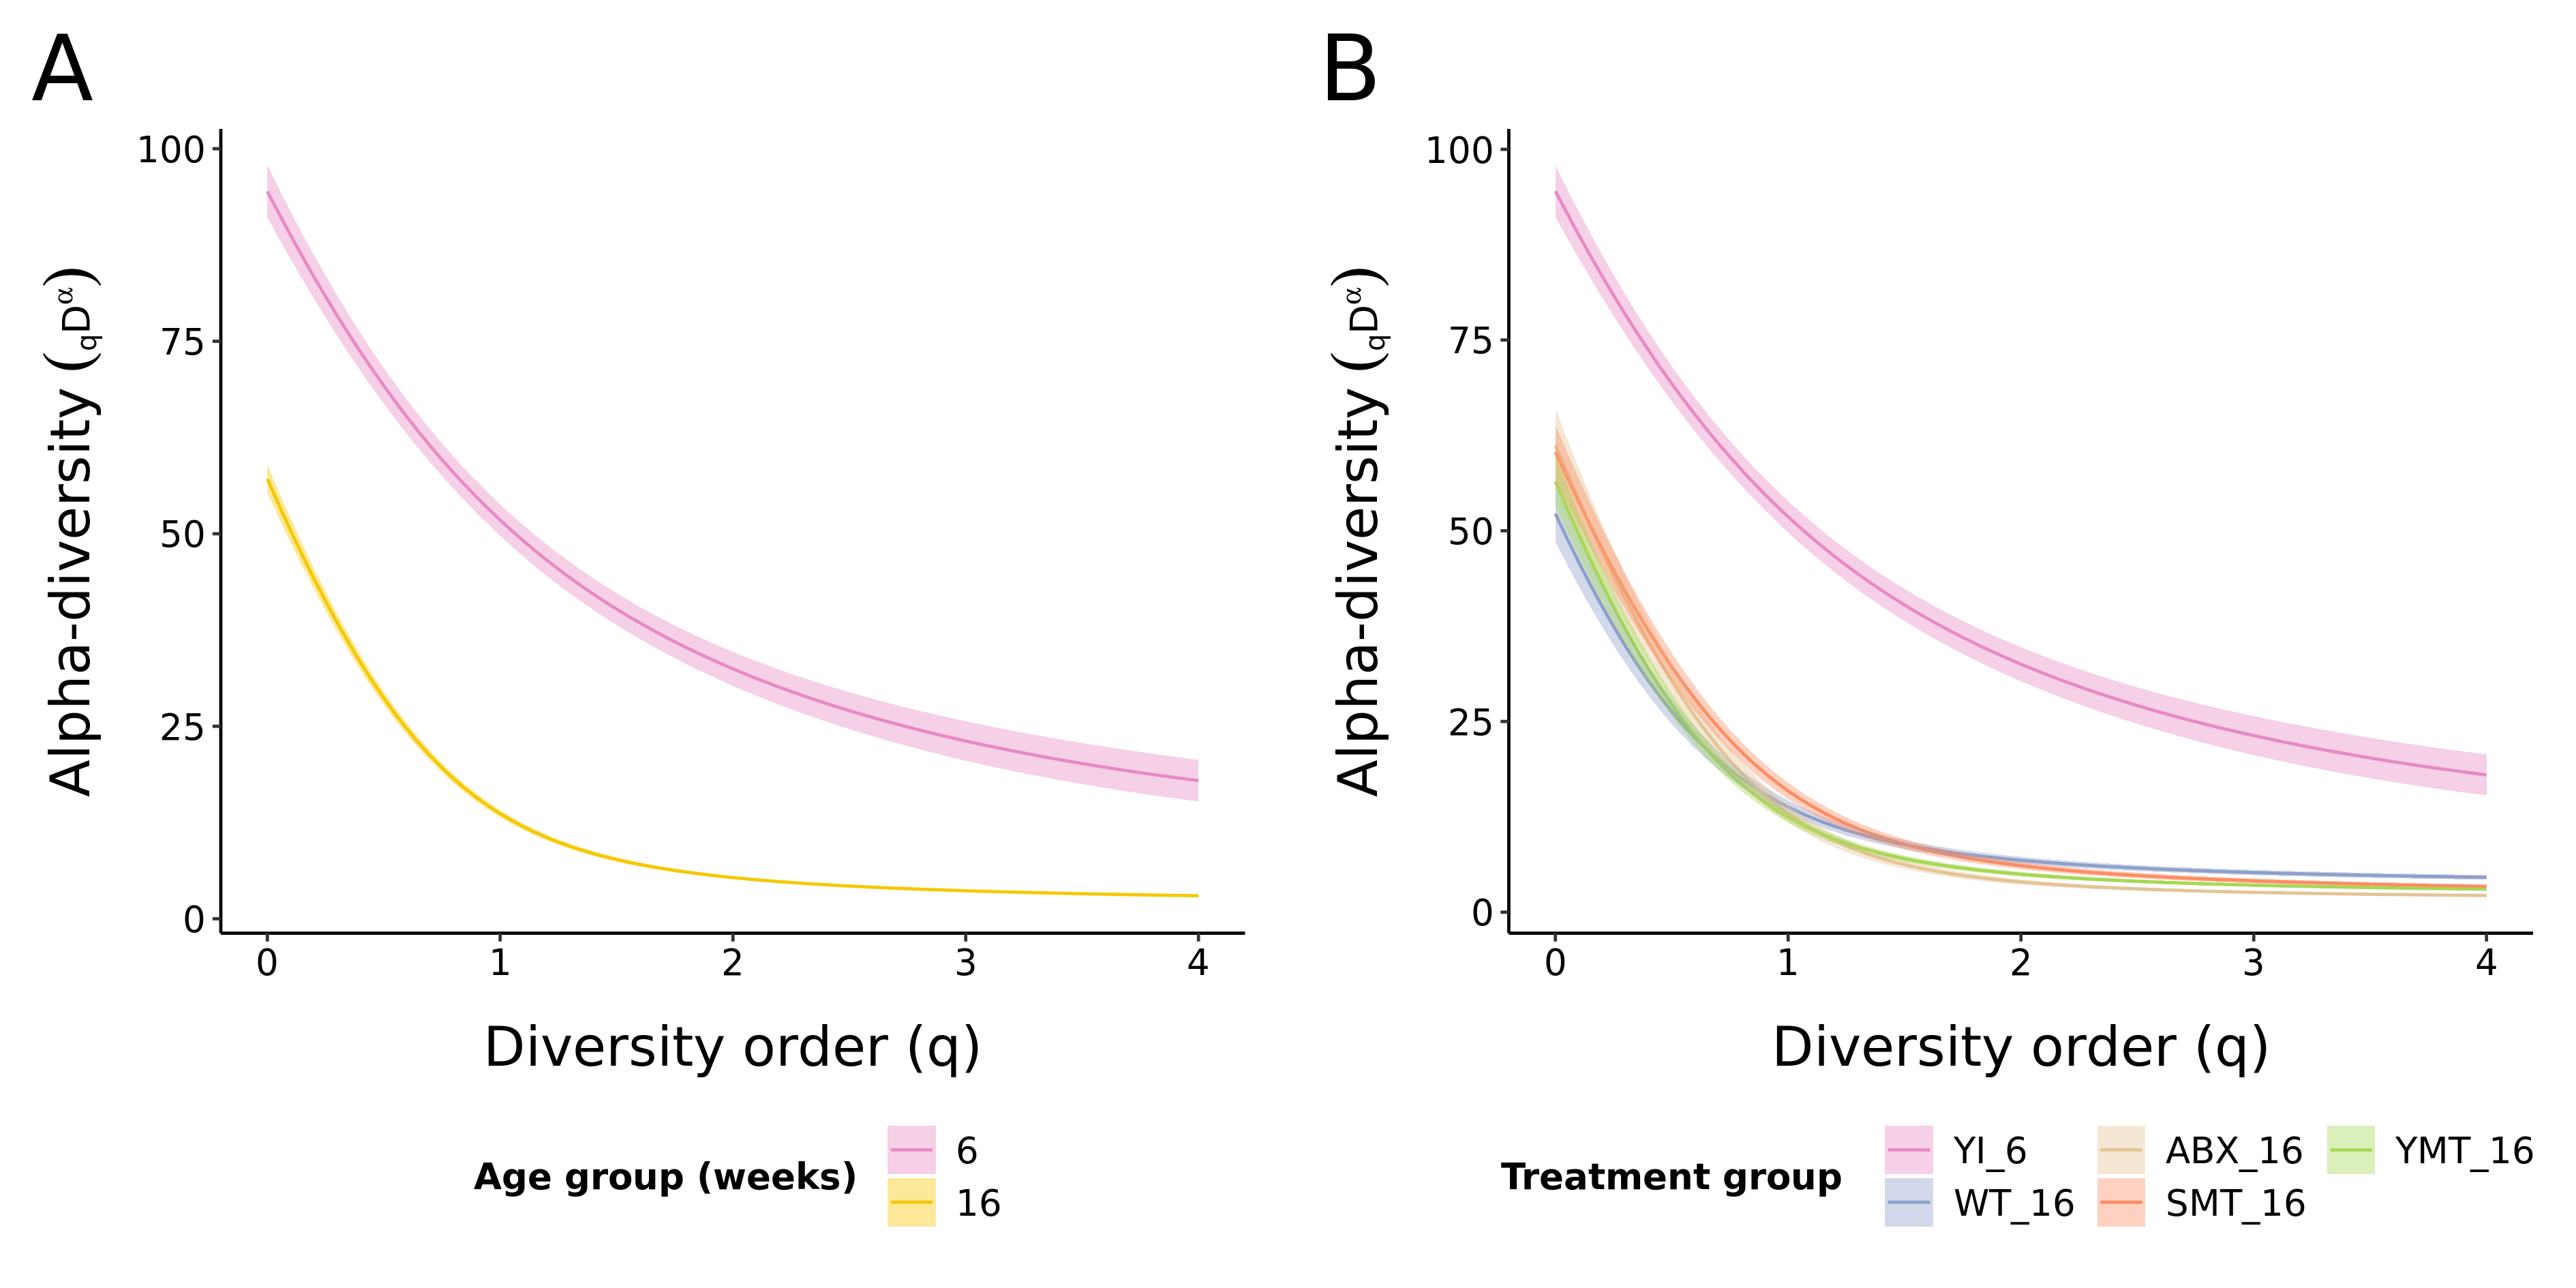
\includegraphics[width = 0.9\textwidth]{_Figures/png/igseq-gut-VJ-diversity-alpha}
\begin{subfigure}{0em}
\phantomsubcaption{}
\label{fig:igseq-gut-VJ-diversity-alpha-age}
\end{subfigure}
\begin{subfigure}{0em}
\phantomsubcaption{}
\label{fig:igseq-gut-VJ-diversity-alpha-groups}
\end{subfigure}
\caption{Bootstrapped alpha-diversity spectra of VJ usage for each (A) age group and (B) treatment group in the \igseq gut dataset, as measured by number of unique sequences per unambiguous VJ identity.}
\label{fig:igseq-gut-VJ-diversity-alpha}
\end{figure}

\begin{figure}
\centering
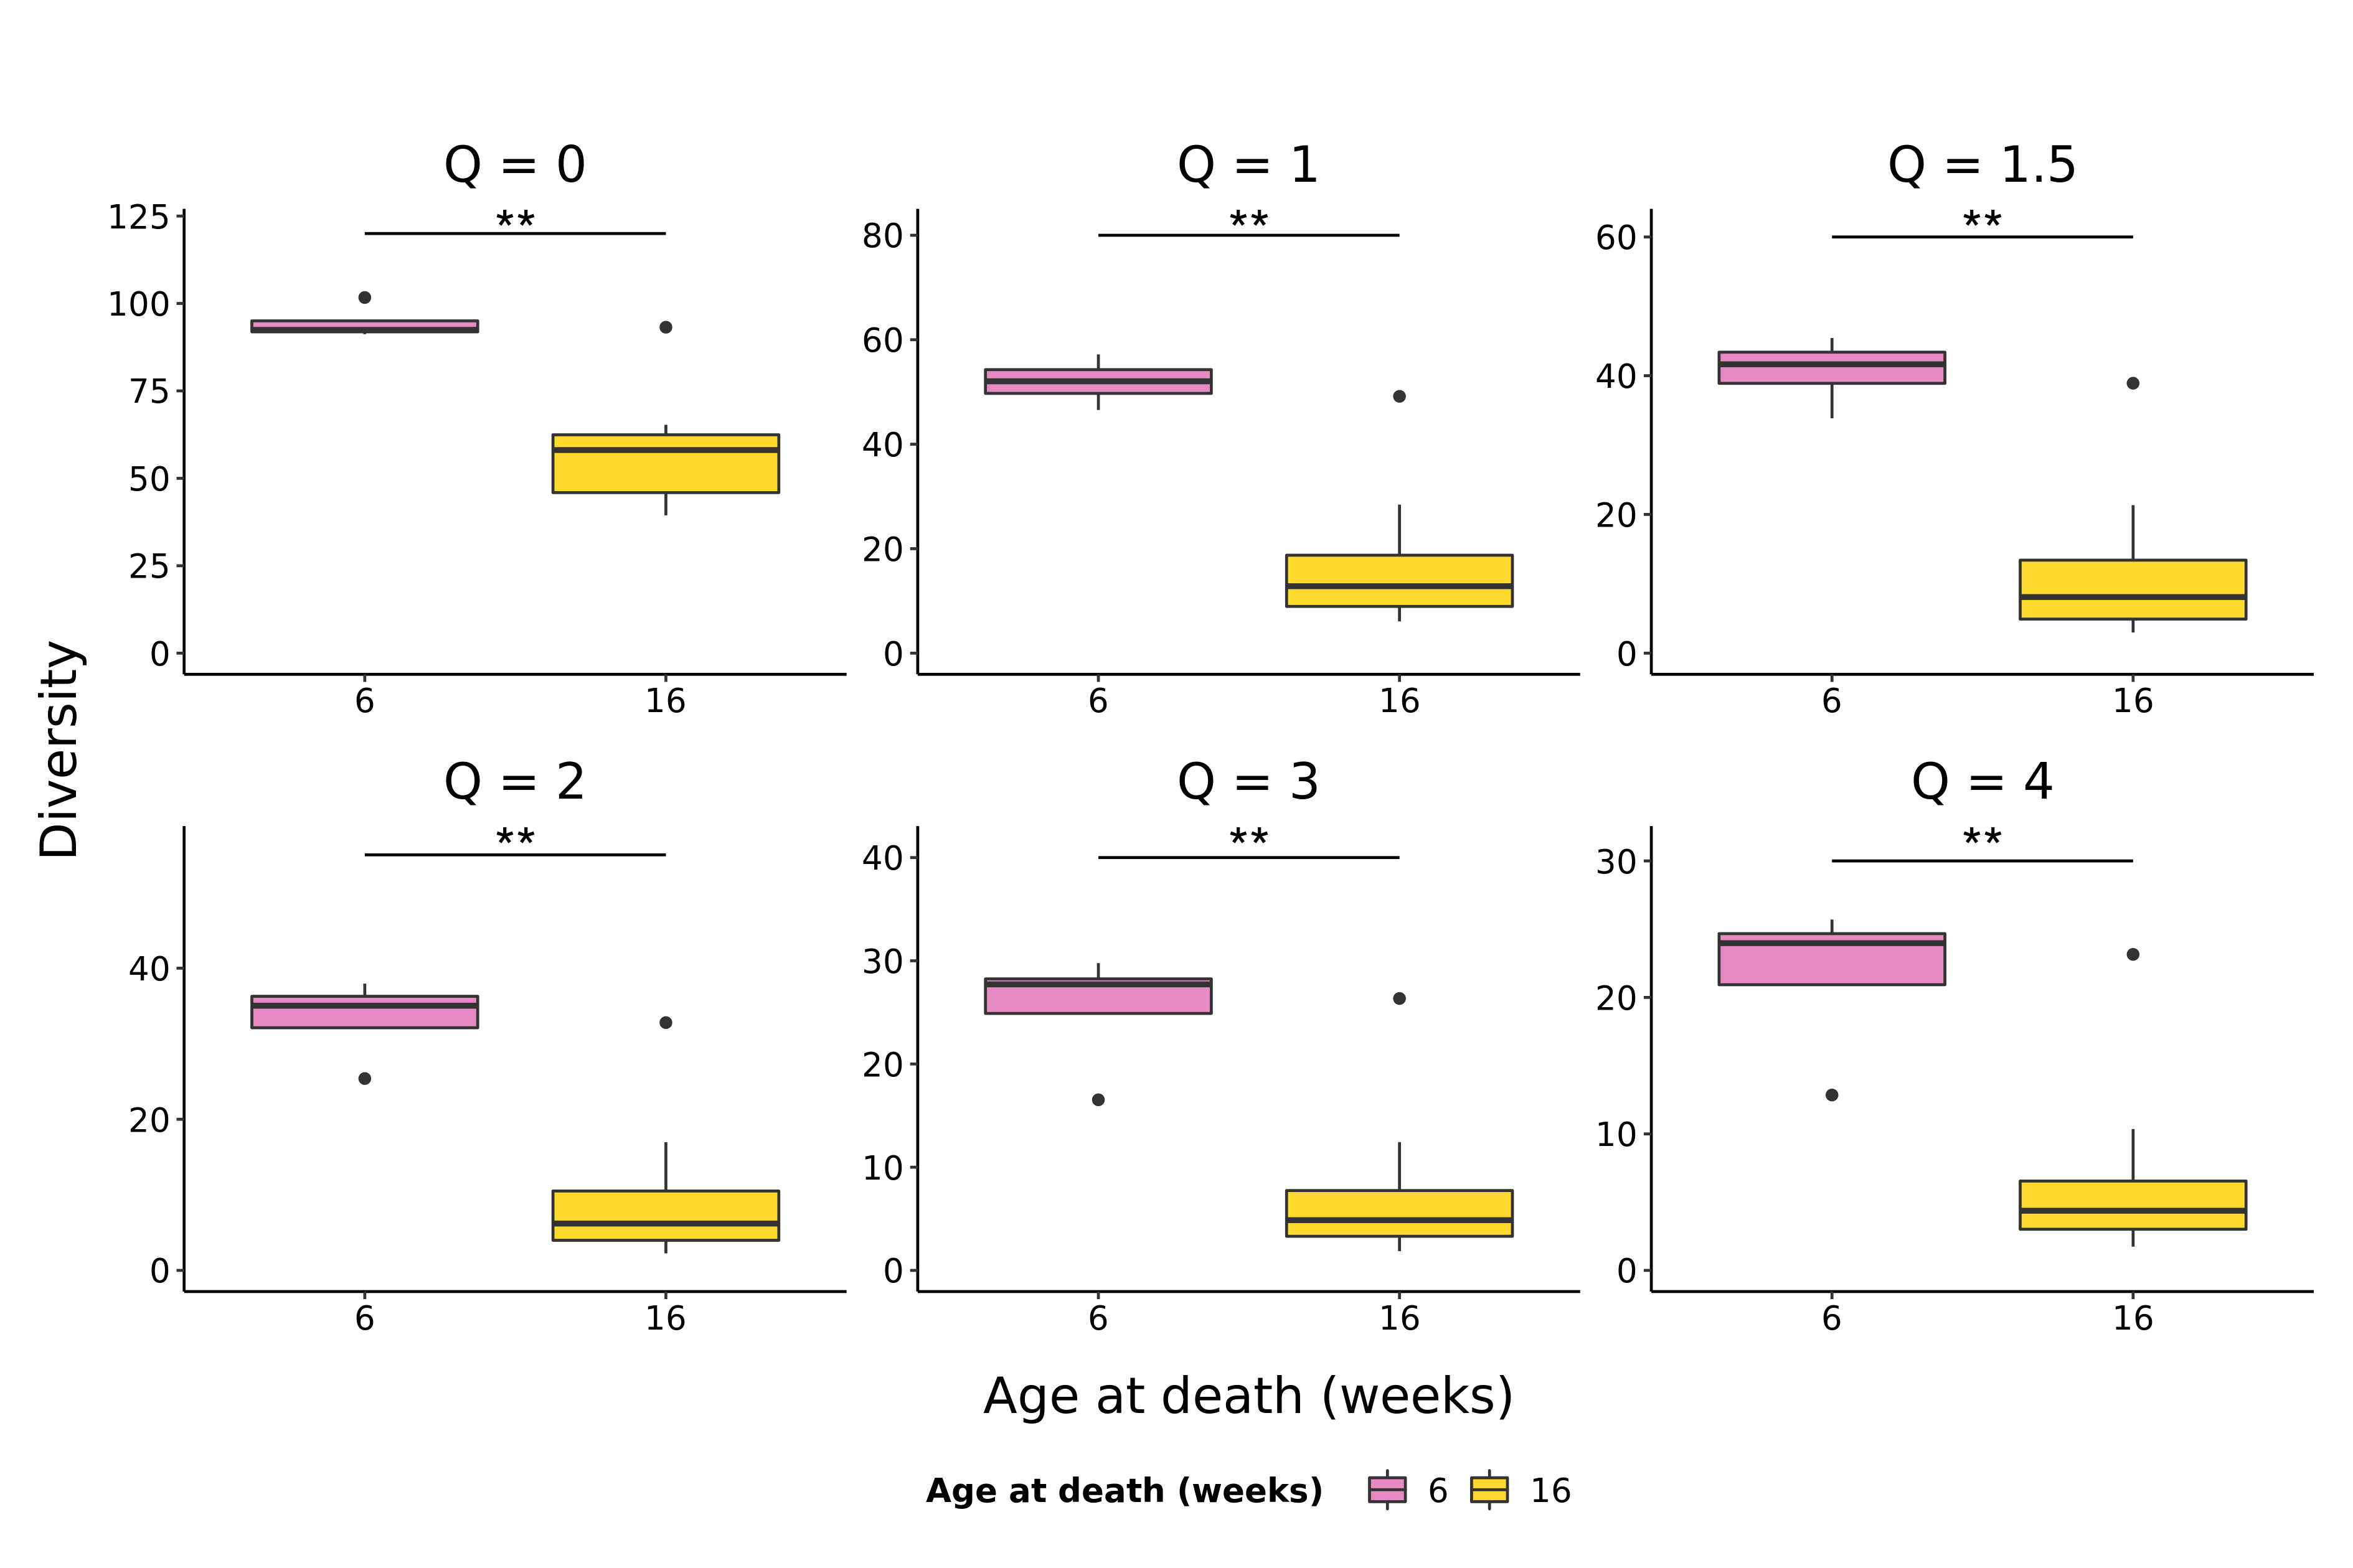
\includegraphics[width = 0.9\textwidth]{_Figures/png/igseq-gut-VJ-diversity-solo-age}
\caption{Boxplots of \textit{VJ} Hill diversity values for the antibody repertoires of individuals of each age group in the \igseq gut dataset at a sample of diversity orders. Pairwise $p$-values are computed using nonparametric Mann–Whitney U tests ($*: 0.01 < p \leq 0.05;~**: 0.001 < p \leq 0.01;~***: p \leq 0.001$).}
\label{fig:igseq-gut-VJ-diversity-solo-age}
\end{figure}

\begin{figure}
\centering
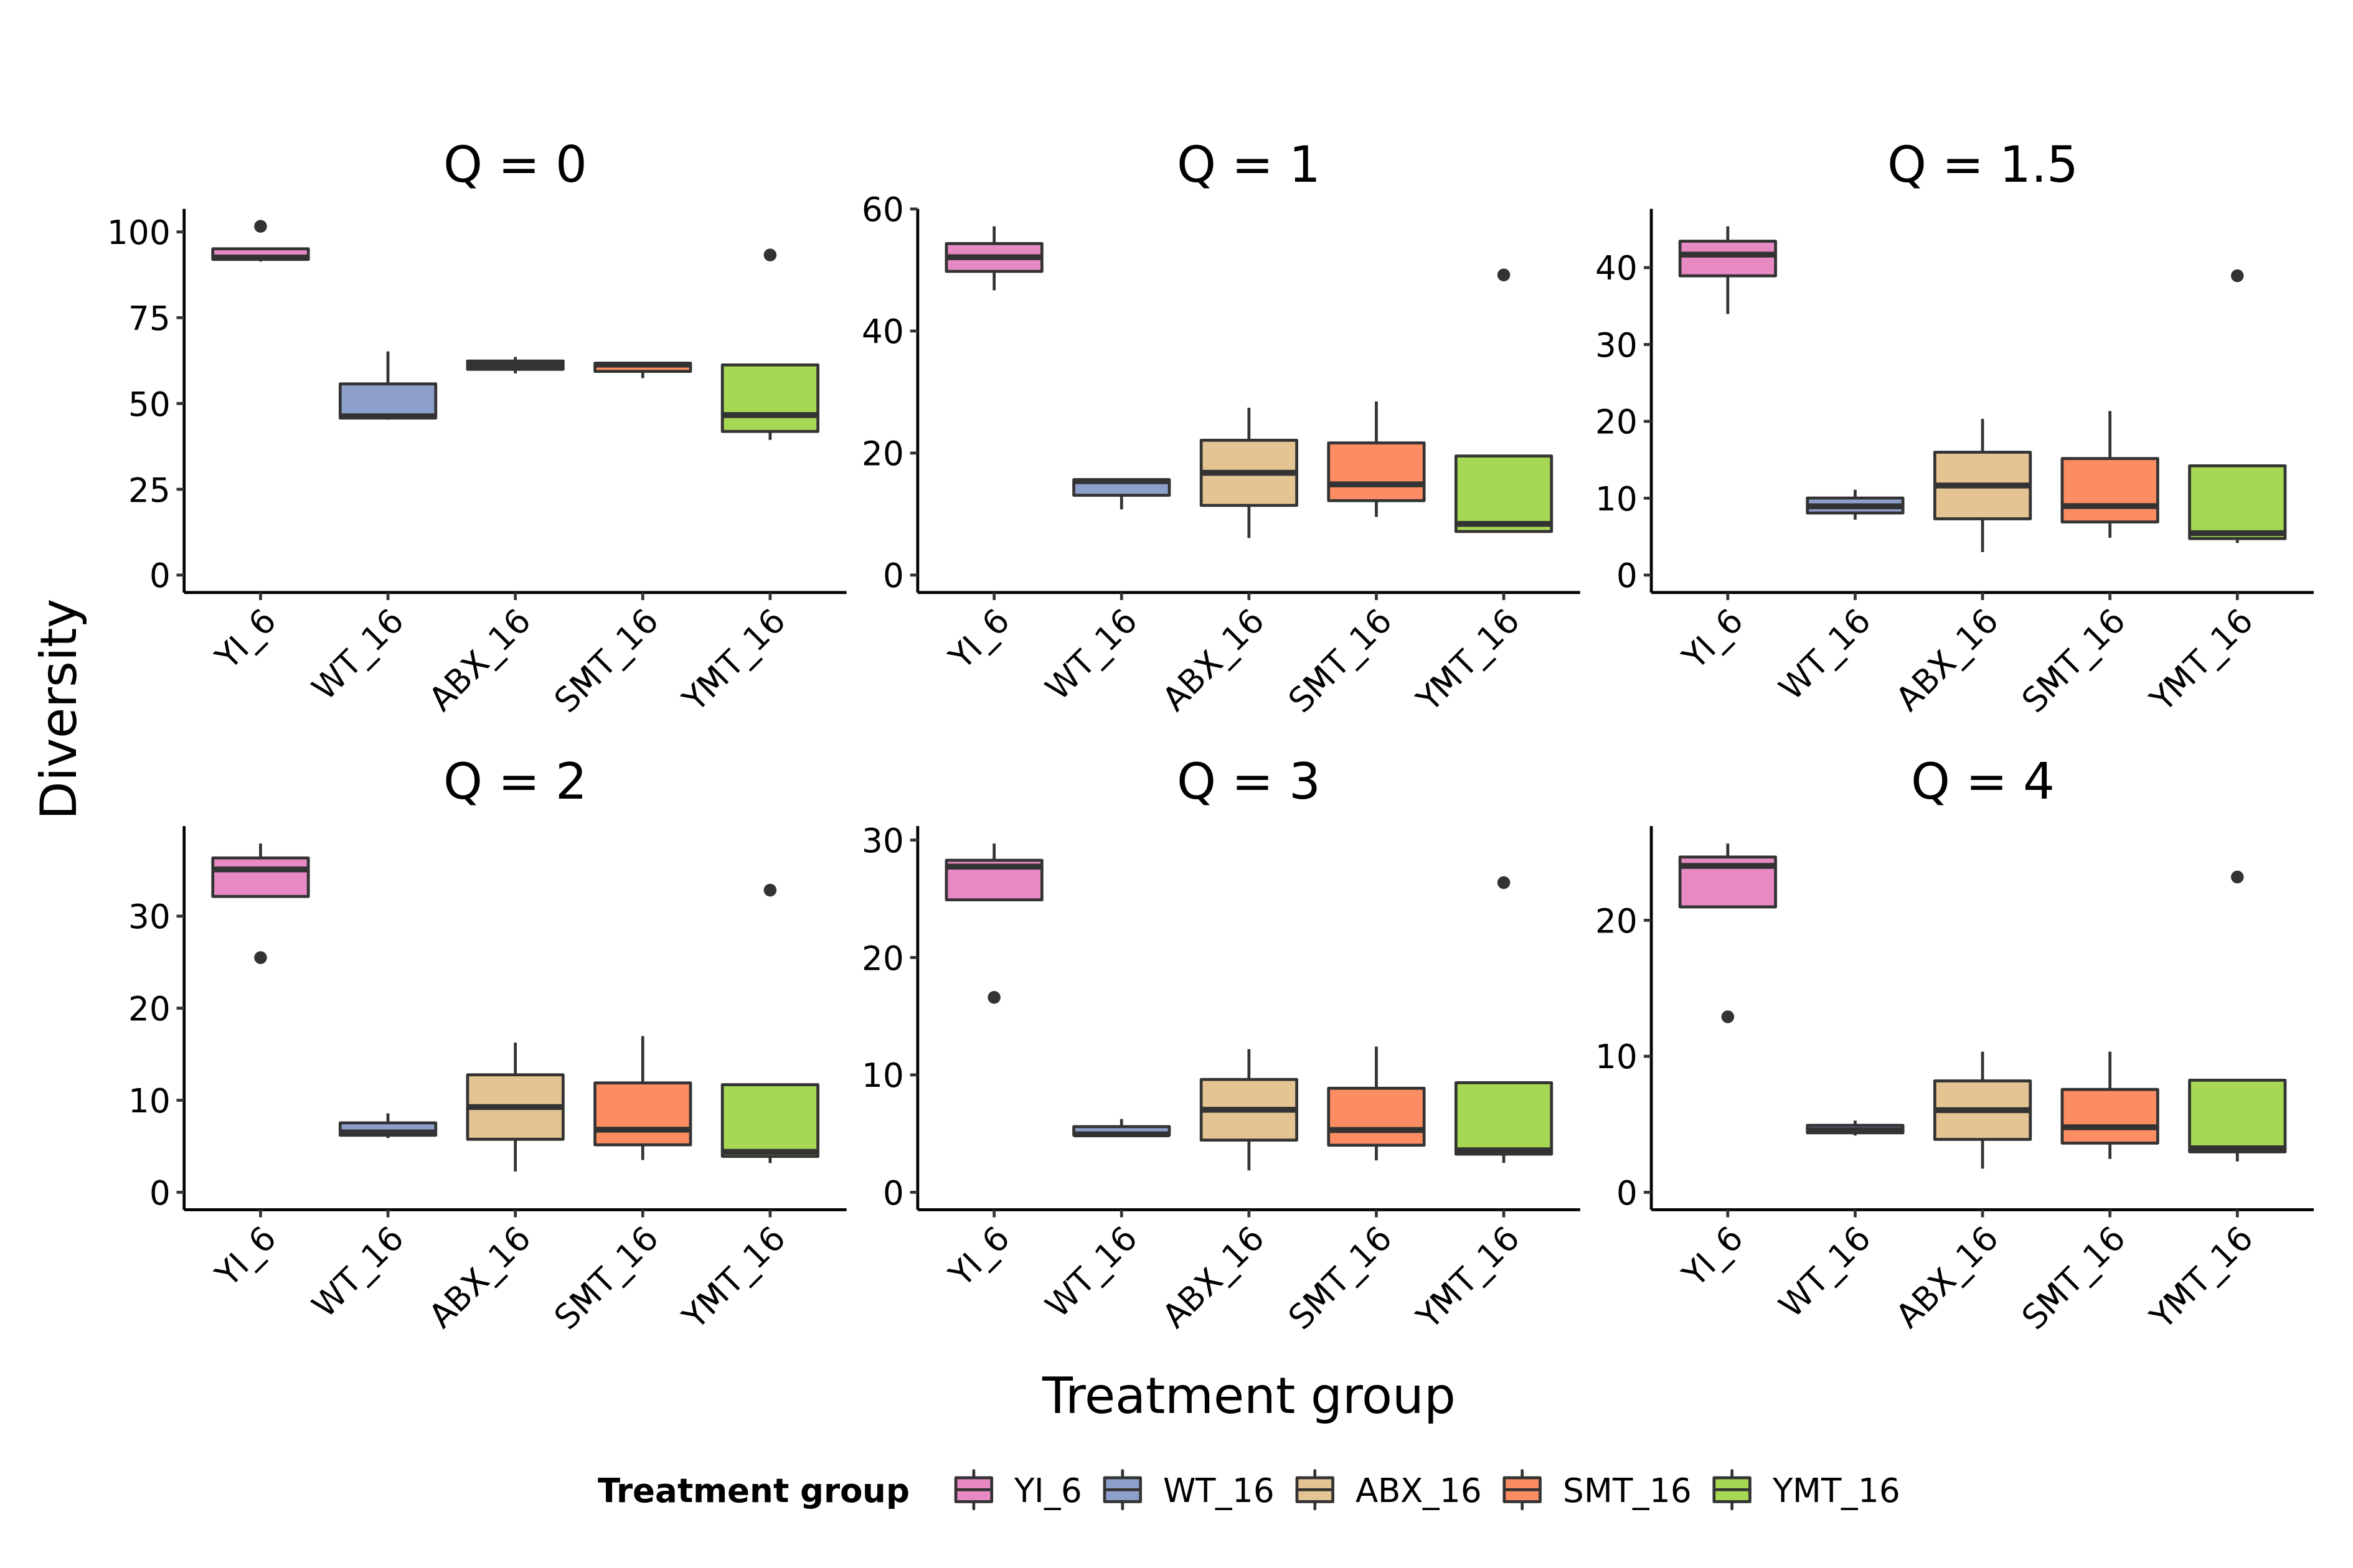
\includegraphics[width = 0.9\textwidth]{_Figures/png/igseq-gut-VJ-diversity-solo-groups}
\caption{Boxplots of \textit{VJ} Hill diversity values for the antibody repertoires of individuals of each treatment group in the \igseq gut dataset at a sample of diversity orders. Pairwise $p$-values are computed using nonparametric Mann–Whitney U tests ($*: 0.01 < p \leq 0.05;~**: 0.001 < p \leq 0.01;~***: p \leq 0.001$).}
\label{fig:igseq-gut-VJ-diversity-solo-groups}
\end{figure}

\begin{figure}
\centering
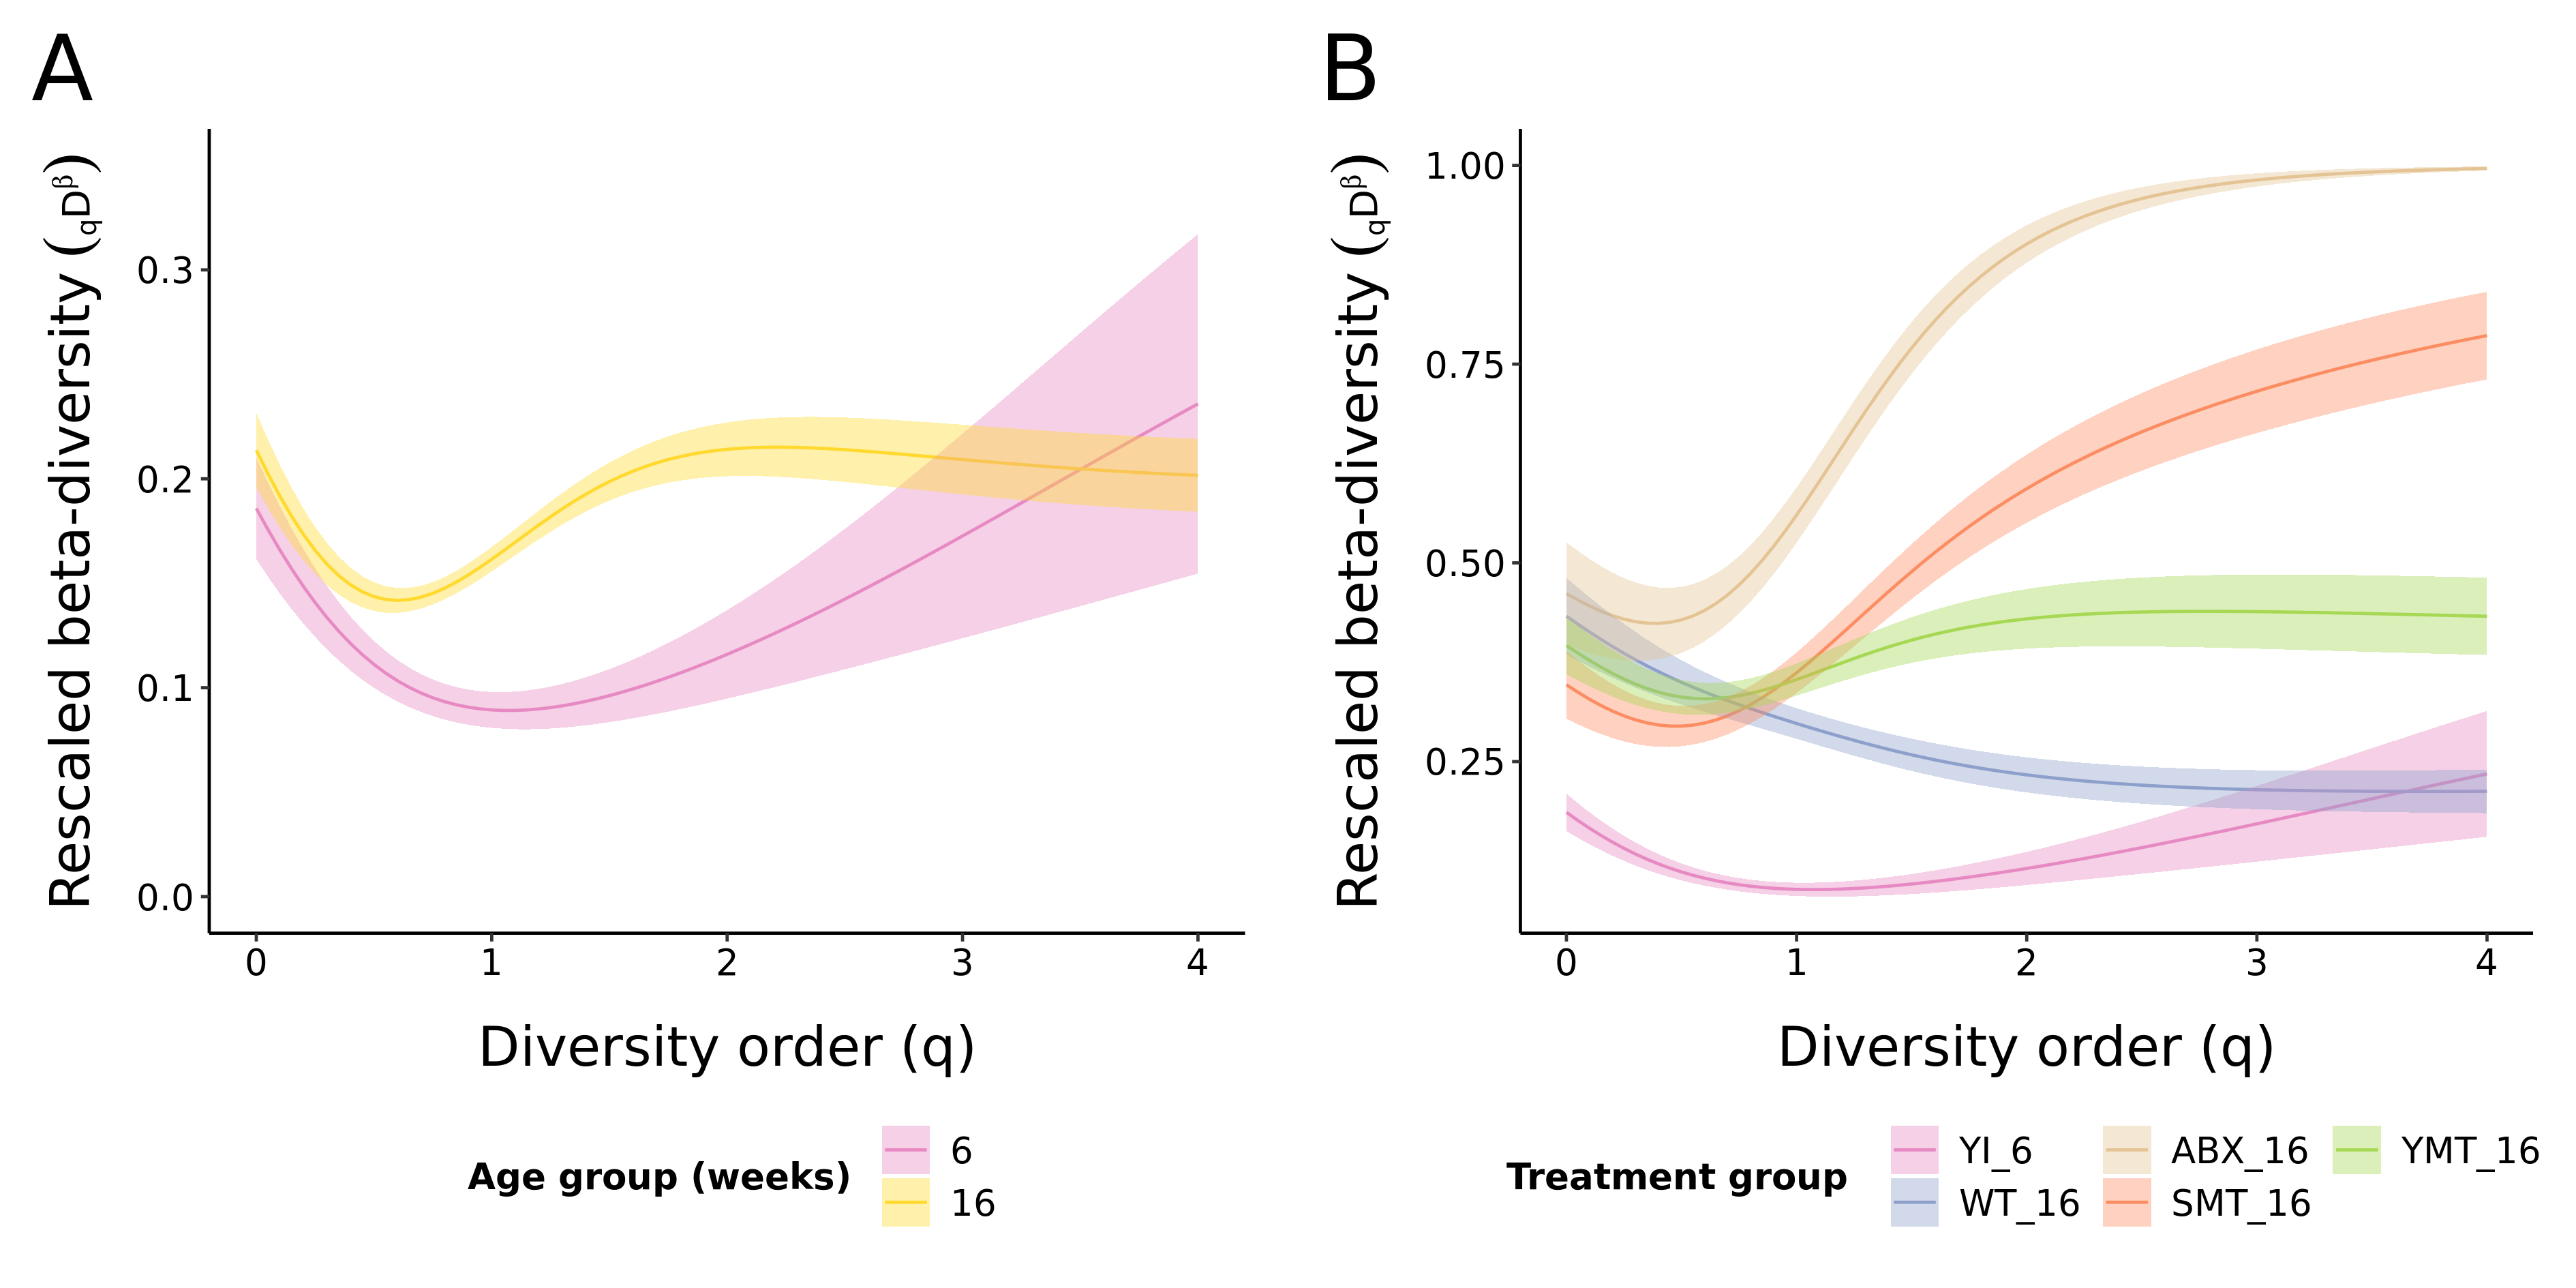
\includegraphics[width = 0.9\textwidth]{_Figures/png/igseq-gut-VJ-diversity-beta}
\begin{subfigure}{0em}
\phantomsubcaption{}
\label{fig:igseq-gut-VJ-diversity-beta-age}
\end{subfigure}
\begin{subfigure}{0em}
\phantomsubcaption{}
\label{fig:igseq-gut-VJ-diversity-beta-groups}
\end{subfigure}
\caption{Bootstrapped beta-diversity spectra of VJ usage, rescaled to between 0 (minimum) and 1 (maximum) for each (A) age group and (B) treatment group in the \igseq gut dataset.}
\label{fig:igseq-gut-VJ-diversity-beta}
\end{figure}


\begin{figure}
\centering
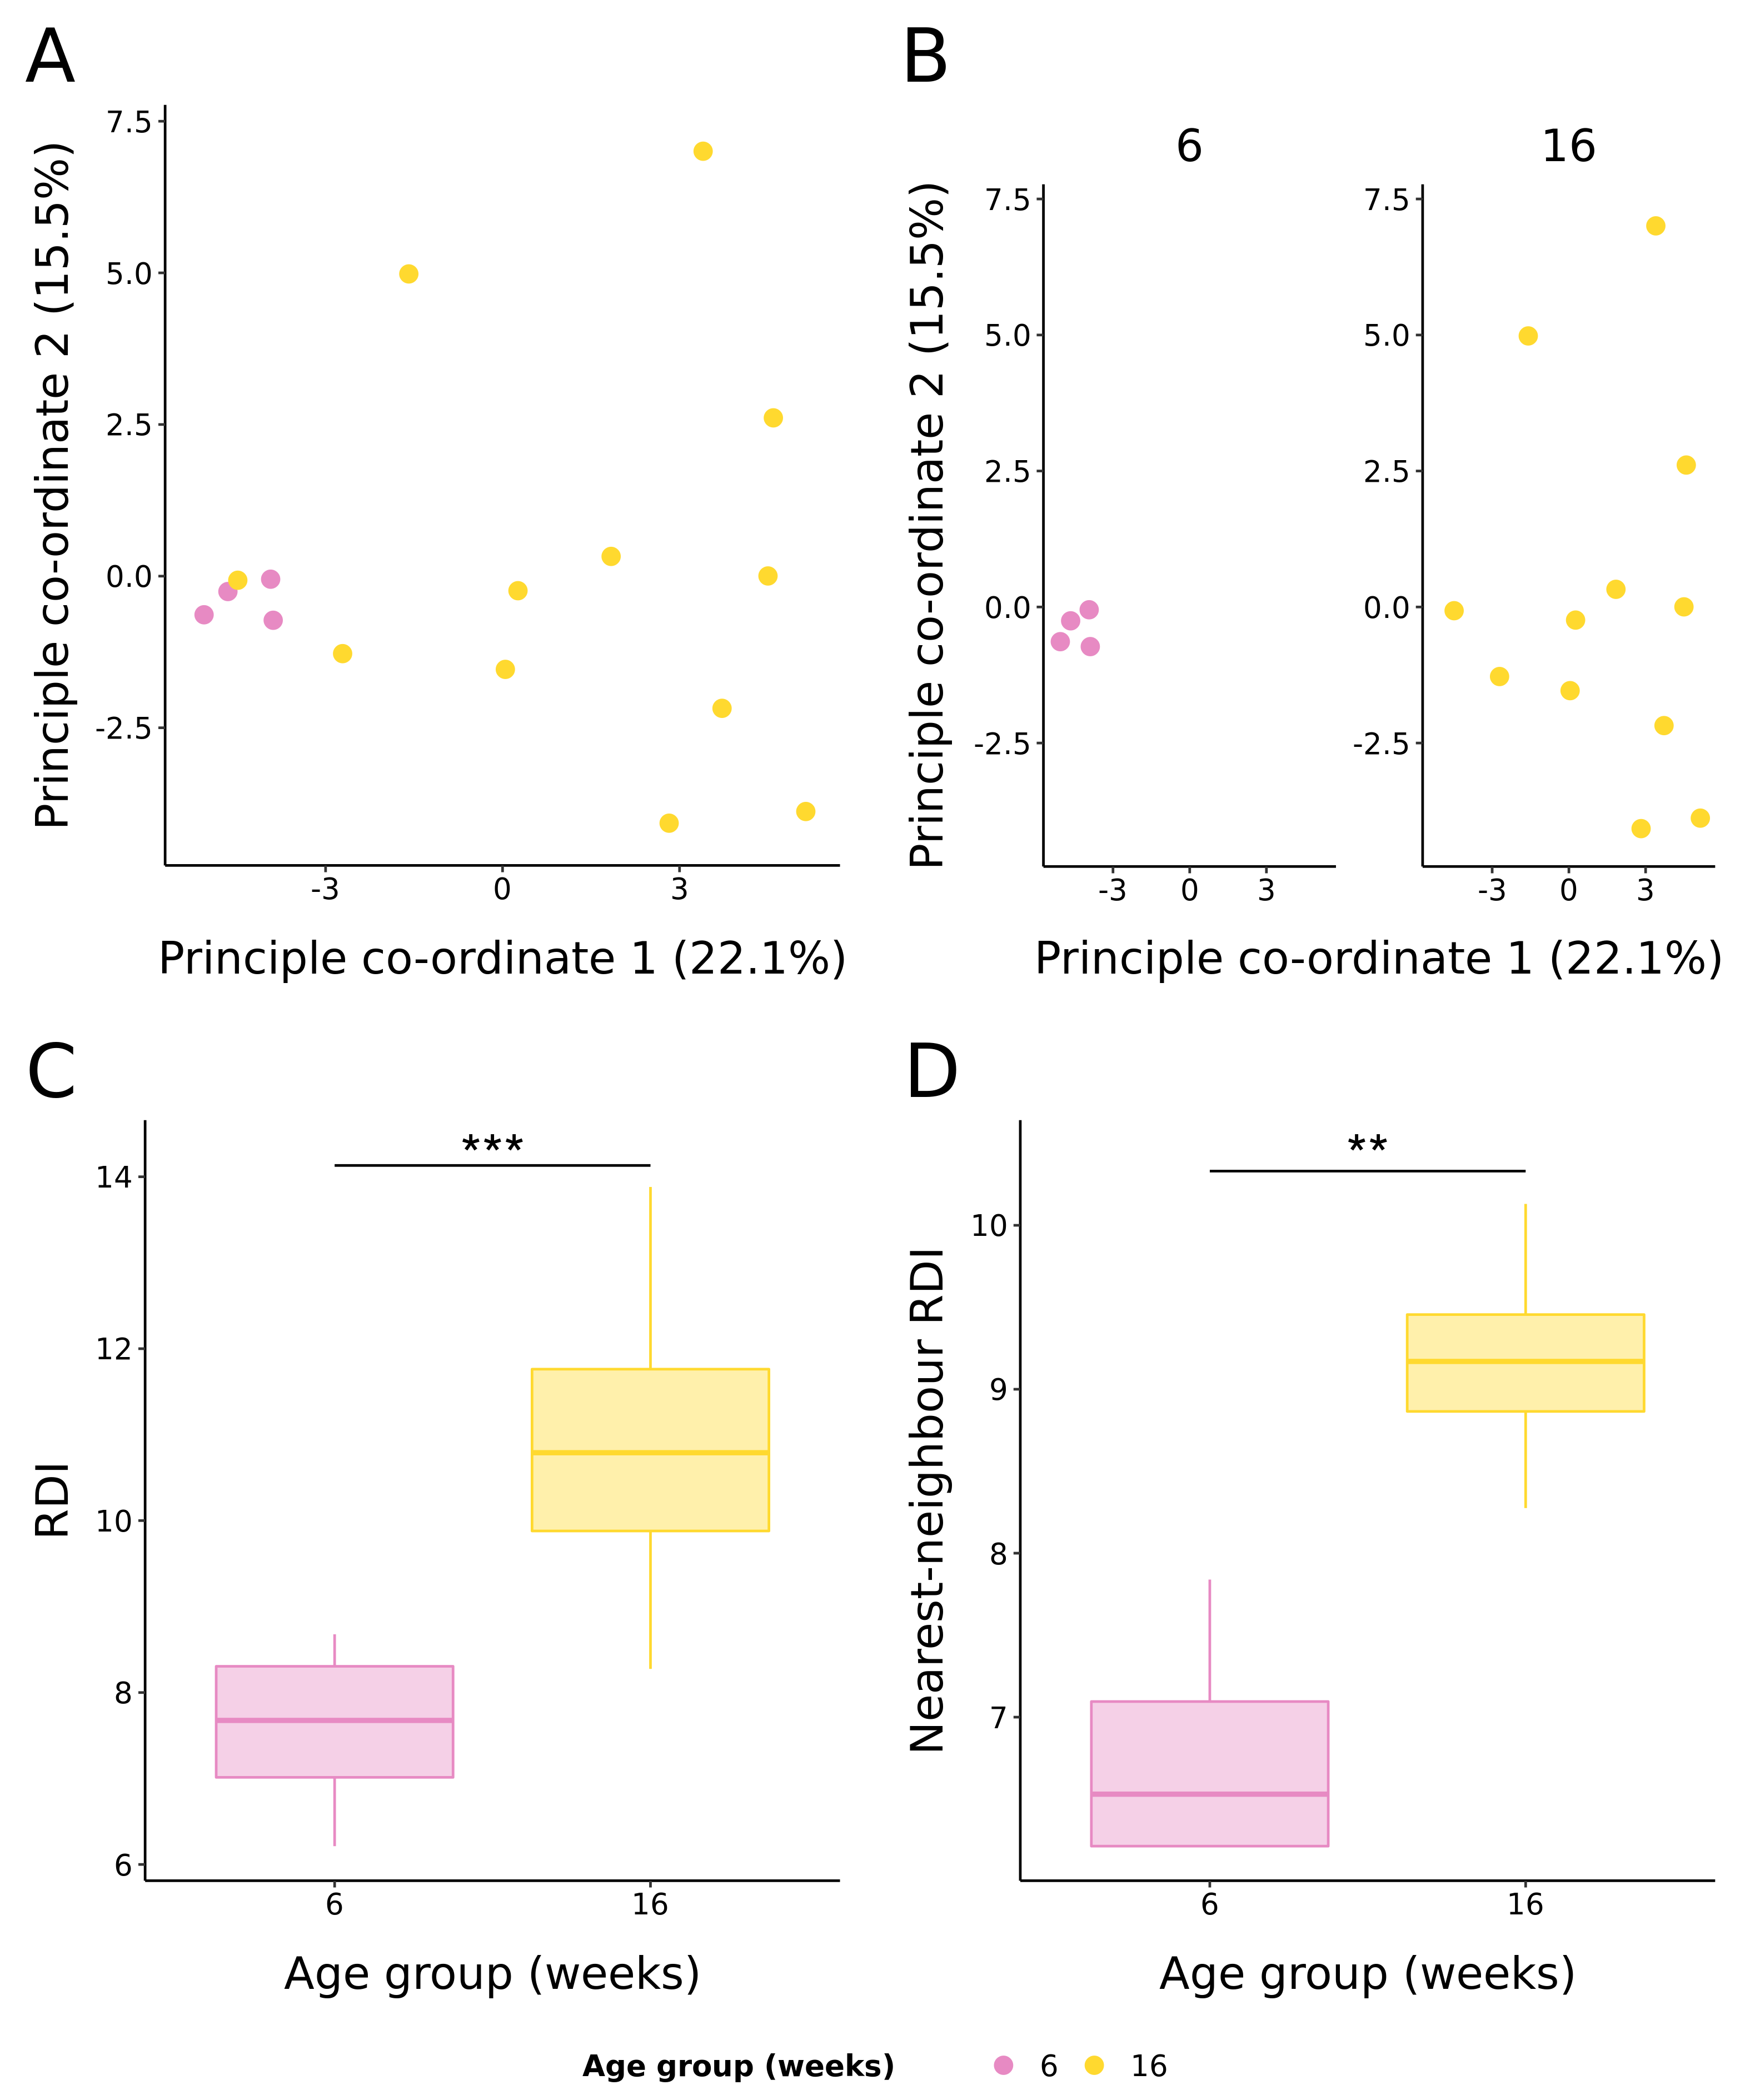
\includegraphics[width = 0.9\textwidth]{_Figures/png/igseq-gut-rdi-VJ-individual-age}
\begin{subfigure}{0em}
\phantomsubcaption{}
\label{fig:igseq-gut-rdi-VJ-individual-age-pcoa-all}
\end{subfigure}
\begin{subfigure}{0em}
\phantomsubcaption{}
\label{fig:igseq-gut-rdi-VJ-individual-age-pcoa-facet}
\end{subfigure}
\begin{subfigure}{0em}
\phantomsubcaption{}
\label{fig:igseq-gut-rdi-VJ-individual-age-groupdist-all}
\end{subfigure}
\begin{subfigure}{0em}
\phantomsubcaption{}
\label{fig:igseq-gut-rdi-VJ-individual-age-groupdist-nn}
\end{subfigure}
\caption{Intra-age-group variability in VJ expression in the \igseq gut dataset. (A-B) Principal co-ordinate analysis (PCoA) of pairwise inter-individual VJ-RDI distances, coloured by age group and displayed together (A) or separately by age group (B). (C-D) Boxplots of overall (C) and nearest-neighbour (D) inter-individual VJ-RDI distances for each age group in the dataset. Pairwise $p$-values are computed using nonparametric Mann–Whitney U tests ($*: 0.01 < p \leq 0.05;~**: 0.001 < p \leq 0.01;~***: p \leq 0.001$).}
\label{fig:igseq-gut-rdi-VJ-individual-age}
\end{figure}

\begin{figure}
\centering
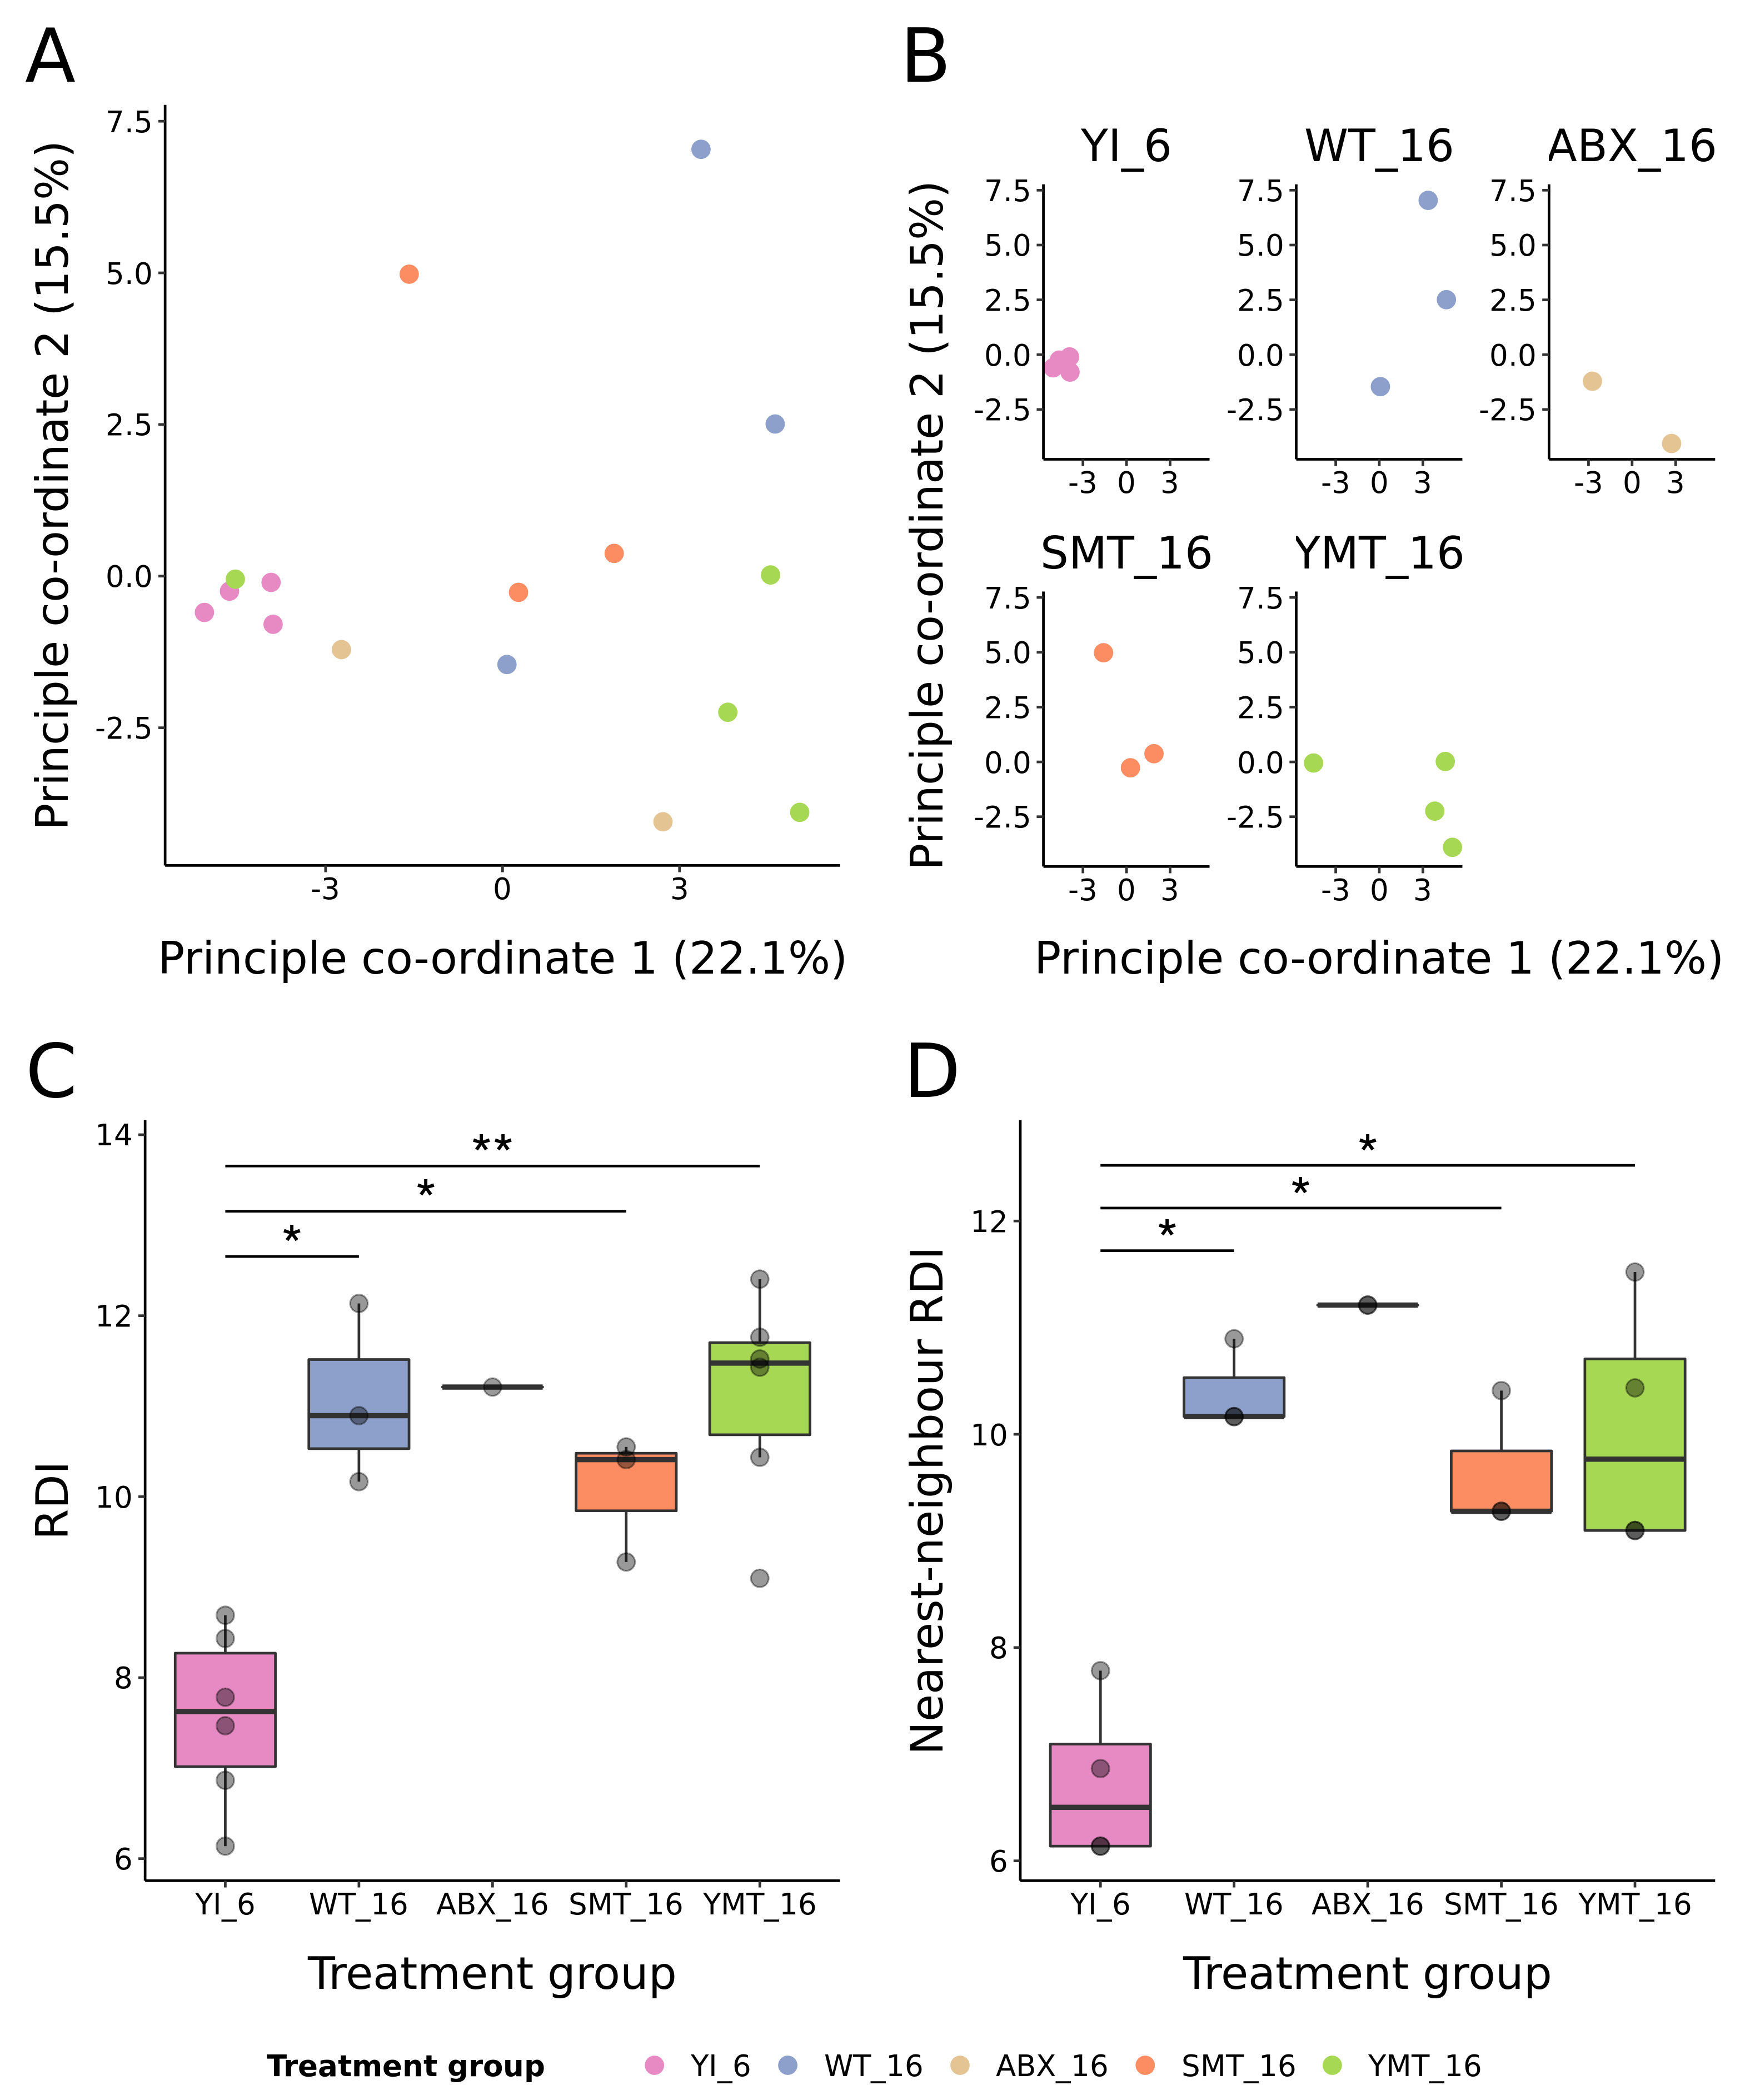
\includegraphics[width = 0.9\textwidth]{_Figures/png/igseq-gut-rdi-VJ-individual-group}
\begin{subfigure}{0em}
\phantomsubcaption{}
\label{fig:igseq-gut-rdi-VJ-individual-group-pcoa-all}
\end{subfigure}
\begin{subfigure}{0em}
\phantomsubcaption{}
\label{fig:igseq-gut-rdi-VJ-individual-group-pcoa-facet}
\end{subfigure}
\begin{subfigure}{0em}
\phantomsubcaption{}
\label{fig:igseq-gut-rdi-VJ-individual-group-groupdist-all}
\end{subfigure}
\begin{subfigure}{0em}
\phantomsubcaption{}
\label{fig:igseq-gut-rdi-VJ-individual-group-groupdist-nn}
\end{subfigure}
\caption{Intra-treatment-group variability in VJ expression in the \igseq gut dataset. (A-B) Principal co-ordinate analysis (PCoA) of pairwise inter-individual VJ-RDI distances, coloured by treatment group and displayed together (A) or separately by treatment group (B). (C-D) Boxplots of overall (C) and nearest-neighbour (D) inter-individual VJ-RDI distances for each treatment group in the dataset. Pairwise $p$-values are computed using nonparametric Mann–Whitney U tests ($*: 0.01 < p \leq 0.05;~**: 0.001 < p \leq 0.01;~***: p \leq 0.001$).}
\label{fig:igseq-gut-rdi-VJ-individual-group}
\end{figure}

These results strongly confirm the changes in killifish repertoire diversity with age observed in section \Cref{sec:igseq_ageing}, with older fish exhibiting a dramatic fall in alpha-diversity and increase in beta-diversity compared to young individuals. The results here are in fact even stronger than those from the whole-body ageing dataset, as there no significant result in VJ alpha-diversity was observed between age groups, while here both VJ and clonal alpha-diversity exhibit a strong and significant decline with age. This difference may result from the lower clonal richness and greater degree of oligoclonality exhibited in gut repertoires: when the local repertoire contains fewer small \naive clones and exhibits a greater degree of domination by the few largest clones, differences in VJ-usage between these large, activated clones may outweigh similar usage distributions in small, \naive clones to a greater extent than in the (much more polyclonal) whole-body repertoire.

% IGOR models: any change in generative distribution with age/treatment?

Conversely, there is no strong evidence from these analyses supporting the hypothesis that gut-microbiota transfer from young fish rejuvenates the antibody repertoire. While the alpha-diversity spectrum of the YMT group appears to be slightly higher than the OMT/ABX groups at very low diversity orders (\Cref{fig:igseq-gut-clone-diversity-alpha-groups}), these indications are not borne out by subsequent statistical analysis, and it is precisely these low-order diversity metrics that are most vulnerable to sampling bias and undersampling (a pervasive problem in \igseq). There is also no obvious difference in VJ alpha-diversity between treatment groups, while the beta-diversity of the YMT group is non-significantly \textit{higher} than that of the untreated control group (\Cref{igseq-gut-VJ-diversity-beta-groups,fig:igseq-gut-rdi-VJ-individual-group-groupdist-all}). Overall, whatever mechanism underlies the effect of gut microbiota transfer on killifish lifespan, it does not appear to be operating through modulation of gut antibody-repertoire diversity. 

\afterpage{%
    \begin{landscape}
        \centering
        \vspace*{\fill}
        \scriptsize
		% latex table generated in R 3.5.2 by xtable 1.8-3 package
% Fri Feb 22 10:04:13 2019
\begin{tabular}{llllll}
  \toprule Fish ID & Age at death (weeks) & Treatment group & Date of library prep & Sequenced? & Reason for exclusion \\ 
  \midrule 1271 & 16 & ABX\_16wk & 2018-11-20 & Yes & -- \\ 
  1274 & 16 & ABX\_16wk & 2018-12-01 & Yes & -- \\ 
  1309 & 16 & ABX\_16wk & 2018-12-01 & Yes & -- \\ 
  dash & 16 & ABX\_16wk & 2018-12-01 & Yes & -- \\ 
  1015 & 16 & SMT\_16wk & 2018-11-20 & Yes & -- \\ 
  1298 & 16 & SMT\_16wk & 2018-11-20 & Yes & -- \\ 
  1301 & 16 & SMT\_16wk & 2018-11-20 & Yes & -- \\ 
  402 & 16 & WT\_16wk & 2018-11-20 & Yes & -- \\ 
  938 & 16 & WT\_16wk & 2018-11-20 & Yes & -- \\ 
  940 & 16 & WT\_16wk & 2018-11-20 & Yes & -- \\ 
  1403 &  6 & YI\_6wk & 2018-11-20 & Yes & -- \\ 
  1409 &  6 & YI\_6wk & 2018-12-01 & Yes & -- \\ 
  1412 &  6 & YI\_6wk & 2018-11-20 & Yes & -- \\ 
  1414 &  6 & YI\_6wk & 2018-11-20 & Yes & -- \\ 
  1009 & 16 & YMT\_16wk & 2018-11-20 & Yes & -- \\ 
  1026 & 16 & YMT\_16wk & 2018-11-20 & Yes & -- \\ 
  1305 & 16 & YMT\_16wk & 2018-11-20 & Yes & -- \\ 
  999 & 16 & YMT\_16wk & 2018-12-01 & Yes & -- \\ 
  400 & 16 & WT\_16wk & -- & No & Not enough RNA for library prep \\ 
  1005 & 16 & SMT\_16wk & -- & No & RNA integrity too low \\ 
   \bottomrule \end{tabular}

		\normalsize\vspace{1em}
        \captionof{table}{Turquoise killifish used in \igseq validation and ageing experiment. All fish are GRZ-Bellemans strain and male.}
        \label{tab:gut-cohorts-fish}
        \vspace*{\fill}
    \end{landscape}
}
% TODO: Try to get detailed information on cohorts (birth and death dates, age in days, etc.)